\chapter{Homotopy type theory}
\label{cha:basics}

The central new idea in homotopy type theory is that types can be regarded as
spaces in homotopy theory, or higher-dimensional groupoids in category
theory.  

\index{classical!homotopy theory|(}
\index{higher category theory|(}
We begin with a brief summary of the connection between homotopy theory
and higher-dimensional category theory.  
In classical homotopy theory, a space $X$ is a set of points equipped
with a topology,
\indexsee{space!topological}{topological space}
\index{topological!space}
and a path between points $x$ and $y$ is represented by
a continuous map $p : [0,1] \to X$, where $p(0) = x$ and $p(1) = y$.
\index{path!topological}
\index{topological!path}
This function can be thought of as giving a point in $X$ at each
``moment in time''.  For many purposes, strict equality of paths
(meaning, pointwise equal functions) is too fine a notion.  For example,
one can define operations of path concatenation (if $p$ is a path from
$x$ to $y$ and $q$ is a path from $y$ to $z$, then the concatenation $p
\ct q$ is a path from $x$ to $z$) and inverses ($\opp p$ is a path
from $y$ to $x$).  However, there are natural equations between these
operations that do not hold for strict equality: for example, the path
$p \ct \opp p$ (which walks from $x$ to $y$, and then back along the
same route, as time goes from $0$ to $1$) is not strictly equal to the
identity path (which stays still at $x$ at all times).

The remedy is to consider a coarser notion of equality of paths called
\emph{homotopy}.
\index{homotopy!topological}
A homotopy between a pair of continuous maps $f :
X_1 \to X_2$ and $g : X_1\to X_2$ is a continuous map $H : X_1
\times [0, 1] \to X_2$ satisfying $H(x, 0) = f (x)$ and $H(x, 1) =
g(x)$.  In the specific case of paths $p$ and $q$ from $x$ to $y$, a homotopy is a
continuous map $H : [0,1] \times [0,1] \rightarrow X$
such that $H(s,0) = p(s)$ and $H(s,1) = q(s)$ for all $s\in [0,1]$.
In this case we require also that $H(0,t) = x$ and $H(1,t)=y$ for all $t\in [0,1]$,
so that for each $t$ the function $H(\blank,t)$ is again a path from $x$ to $y$;
a homotopy of this sort is said to be \emph{endpoint-preserving} or \emph{rel endpoints}.
Such a homotopy is the
image in $X$ of a square that fills in the space between $p$ and $q$,
which can be thought of as a ``continuous deformation'' between $p$ and
$q$, or a 2-dimensional \emph{path between paths}.\index{path!2-}

For example, because
$p \ct \opp p$ walks out and back along the same route, you know that
you can continuously shrink $p \ct \opp p$ down to the identity
path---it won't, for example, get snagged around a hole in the space.
Homotopy is an equivalence relation, and operations such as
concatenation, inverses, etc., respect it.  Moreover, the homotopy
equivalence classes of loops\index{loop} at some point $x_0$ (where two loops $p$
and $q$ are equated when there is a \emph{based} homotopy between them,
which is a homotopy $H$ as above that additionally satisfies $H(0,t) =
H(1,t) = x_0$ for all $t$) form a group called the \emph{fundamental
  group}.\index{fundamental!group}  This group is an \emph{algebraic invariant} of a space, which
can be used to investigate whether two spaces are \emph{homotopy
  equivalent} (there are continuous maps back and forth whose composites
are homotopic to the identity), because equivalent spaces have
isomorphic fundamental groups.

Because homotopies are themselves a kind of 2-dimensional path, there is
a natural notion of 3-dimensional \emph{homotopy between homotopies},\index{path!3-}
and then \emph{homotopy between homotopies between homotopies}, and so
on.  This infinite tower of points, path, homotopies, homotopies between
homotopies, \ldots, equipped with algebraic operations such as the
fundamental group, is an instance of an algebraic structure called a
(weak) \emph{$\infty$-groupoid}.  An $\infty$-groupoid\index{.infinity-groupoid@$\infty$-groupoid} consists of a
collection of objects, and then a collection of \emph{morphisms}\indexdef{morphism!in an .infinity-groupoid@in an $\infty$-groupoid} between
objects, and then \emph{morphisms between morphisms}, and so on,
equipped with some complex algebraic structure; a morphism at level $k$ is called a \define{$k$-morphism}\indexdef{k-morphism@$k$-morphism}.  Morphisms at each level
have identity, composition, and inverse operations, which are weak in
the sense that they satisfy the groupoid laws (associativity of
composition, identity is a unit for composition, inverses cancel) only
up to morphisms at the next level, and this weakness gives rise to
further structure. For example, because associativity of composition of
morphisms $p \ct (q \ct r) = (p \ct q) \ct r$ is itself a
higher-dimensional morphism, one needs an additional operation relating
various proofs of associativity: the various ways to reassociate $p \ct
(q \ct (r \ct s))$ into $((p \ct q) \ct r) \ct s$ give rise to Mac
Lane's pentagon\index{pentagon, Mac Lane}.  Weakness also creates non-trivial interactions between
levels.

Every topological space $X$ has a \emph{fundamental $\infty$-groupoid}
\index{.infinity-groupoid@$\infty$-groupoid!fundamental}
\index{fundamental!.infinity-groupoid@$\infty$-groupoid}
whose
$k$-mor\-ph\-isms are the $k$-dimen\-sional paths in $X$.  The weakness of the
$\infty$-group\-oid corresponds directly to the fact that paths form a
group only up to homotopy, with the $(k+1)$-paths serving as the
homotopies between the $k$-paths.  Moreover, the view of a space as an
$\infty$-groupoid preserves enough aspects of the space to do homotopy theory:
the fundamental $\infty$-groupoid construction is adjoint\index{adjoint!functor} to the
geometric\index{geometric realization} realization of an $\infty$-groupoid as a space, and this
adjunction preserves homotopy theory (this is called the \emph{homotopy
  hypothesis/theorem},
\index{hypothesis!homotopy}
\index{homotopy!hypothesis}
because whether it is a hypothesis or theorem
depends on how you define $\infty$-groupoid).  For example, you can
easily define the fundamental group of an $\infty$-groupoid, and if you
calculate the fundamental group of the fundamental $\infty$-groupoid of
a space, it will agree with the classical definition of fundamental
group of that space.  Because of this correspondence, homotopy theory
and higher-dimensional category theory are intimately related.

\index{classical!homotopy theory|)}%
\index{higher category theory|)}%

\mentalpause

Now, in homotopy type theory each type can be seen to have the structure
of an $\infty$-groupoid.  Recall that for any type $A$, and any $x,y:A$,
we have a identity type $\id[A]{x}{y}$, also written $\idtype[A]{x}{y}$
or just $x=y$.  Logically, we may think of elements of $x=y$ as evidence
that $x$ and $y$ are equal, or as identifications of $x$ with
$y$. Furthermore, type theory (unlike, say, first-order logic) allows us
to consider such elements of $\id[A]{x}{y}$ also as individuals which
may be the subjects of further propositions.  Therefore, we can
\emph{iterate} the identity type: we can form the type
$\id[{(\id[A]{x}{y})}]{p}{q}$ of identifications between
identifications $p,q$, and the type
$\id[{(\id[{(\id[A]{x}{y})}]{p}{q})}]{r}{s}$, and so on.  The structure
of this tower of identity types corresponds precisely to that of the
continuous paths and (higher) homotopies between them in a space, or an
$\infty$-groupoid.\index{.infinity-groupoid@$\infty$-groupoid}


Thus, we will frequently refer to an element $p : \id[A]{x}{y}$ as
a \define{path}
\index{path}
from $x$ to $y$; we call $x$ its \define{start point}
\indexdef{start point of a path}
\indexdef{path!start point of}
and $y$ its \define{end point}.
\indexdef{end point of a path}
\indexdef{path!end point of}
Two paths $p,q : \id[A]{x}{y}$ with the same start and end point are said to be \define{parallel},
\indexdef{parallel paths}
\indexdef{path!parallel}
in which case an element $r : \id[{(\id[A]{x}{y})}]{p}{q}$ can
be thought of as a homotopy, or a morphism between morphisms;
we will often refer to it as a \define{2-path}
\indexdef{path!2-}\indexsee{2-path}{path, 2-}%
or a \define{2-dimensional path}
\index{dimension!of paths}%
\indexsee{2-dimensional path}{path, 2-}\indexsee{path!2-dimensional}{path, 2-}%
Similarly, $\id[{(\id[{(\id[A]{x}{y})}]{p}{q})}]{r}{s}$ is the type of
\define{3-dimensional paths}
\indexdef{path!3-}\indexsee{3-path}{path, 3-}\indexsee{3-dimensional path}{path, 3-}\indexsee{path!3-dimensional}{path, 3-}%
between two parallel 2-dimensional paths, and so on.  If the
type $A$ is ``set-like'', such as \nat, these iterated identity types
will be uninteresting (see \autoref{sec:basics-sets}), but in the
general case they can model non-trivial homotopy types.

%% (Obviously, the
%% notation ``$\id[A]{x}{y}$'' has its limitations here.  The style
%% $\idtype[A]{x}{y}$ is only slightly better in iterations:
%% $\idtype[{\idtype[{\idtype[A]{x}{y}}]{p}{q}}]{r}{s}$.)

An important difference between homotopy type theory and classical homotopy theory is that homotopy type theory provides a \emph{synthetic}
\index{synthetic mathematics}%
\index{geometry, synthetic}%
\index{Euclid of Alexandria}%
description of spaces, in the following sense. Synthetic geometry is geometry in the style of Euclid~\cite{Euclid}: one starts from some basic notions (points and lines), constructions (a line connecting any two points), and axioms
(all right angles are equal), and deduces consequences logically.  This is in contrast with analytic
\index{analytic mathematics}%
geometry, where notions such as points and lines are represented concretely using cartesian coordinates in $\R^n$---lines are sets of points---and the basic constructions and axioms are derived from this representation.  While classical homotopy theory is analytic (spaces and paths are made of points), homotopy type theory is synthetic: points, paths, and paths between paths are basic, indivisible, primitive notions.

Moreover, one of the amazing things about homotopy type theory is that all of the basic constructions and axioms---all of the
higher groupoid structure----arises automatically from the induction
principle for identity types.
Recall from \autoref{sec:identity-types} that this says that if
\begin{itemize}
\item for every $x,y:A$ and every $p:\id[A]xy$ we have a type $D(x,y,p)$, and
\item for every $a:A$ we have an element $d(a):D(a,a,\refl a)$, 
\end{itemize}
then
\begin{itemize}
\item there exists an element $\indid{A}(D,d,x,y,p):D(x,y,p)$ for \emph{every} two elements $x,y:A$ and $p:\id[A]xy$, such that $\indid{A}(D,d,a,a,\refl a) \jdeq d(a)$.
\end{itemize}
In other words, given dependent functions
\begin{align*}
D & :\prd{x,y:A}{p:\id{x}{y}} \type\\
d & :\prd{a:A} D(a,a,\refl{a})
\end{align*}
there is a dependent function
\[\indid{A}(D,d):\prd{x,y:A}{p:\id{x}{y}} D(x,y,p)\]
such that 
\begin{equation}\label{eq:Jconv}
\indid{A}(D,d,a,a,\refl{a})\jdeq d(a)
\end{equation}
for every $a:A$.
Usually, every time we apply this induction rule we will either not care about the specific function being defined, or we will immediately give it a different name.

Informally, the induction principle for identity types says that if we want to construct an object (or prove a statement) which depends on an inhabitant $p:\id[A]xy$ of an identity type, then it suffices to perform the construction (or the proof) in the special case when $x$ and $y$ are the same (judgmentally) and $p$ is the reflexivity element $\refl{x}:x=x$ (judgmentally).
When writing informally, we may express this with a phrase such as ``by induction, it suffices to assume\dots''.
This reduction to the ``reflexivity case'' is analogous to the reduction to the ``base case'' and ``inductive step'' in an ordinary proof by induction on the natural numbers, and also to the ``left case'' and ``right case'' in a proof by case analysis on a disjoint union or disjunction.\index{induction principle!for identity type}%


The ``conversion rule''~\eqref{eq:Jconv} is less familiar in the context of proof by induction on natural numbers, but there is an analogous notion in the related concept of definition by recursion.
If a sequence\index{sequence} $(a_n)_{n\in \mathbb{N}}$ is defined by giving $a_0$ and specifying $a_{n+1}$ in terms of $a_n$, then in fact the $0^{\mathrm{th}}$ term of the resulting sequence \emph{is} the given one, and the given recurrence relation relating $a_{n+1}$ to $a_n$ holds for the resulting sequence.
(This may seem so obvious as to not be worth saying, but if we view a definition by recursion as an algorithm\index{algorithm} for calculating values of a sequence, then it is precisely the process of executing that algorithm.)
The rule~\eqref{eq:Jconv} is analogous: it says that if we define an object $f(p)$ for all $p:x=y$ by specifying what the value should be when $p$ is $\refl{x}:x=x$, then the value we specified is in fact the value of $f(\refl{x})$.

This induction principle endows each type with the structure of an $\infty$-groupoid\index{.infinity-groupoid@$\infty$-groupoid}, and each function between two types the structure of an $\infty$-functor\index{.infinity-functor@$\infty$-functor} between two such groupoids.  This is interesting from a mathematical point of view, because it gives a new way to work with
$\infty$-groupoids.  It is interesting from a type-theoretic point of view, because it reveals new operations that are associated with each type and function.  In the remainder of this chapter, we begin to explore this structure.

\section{Types are higher groupoids}
\label{sec:equality}

\index{type!identity|(}%
\index{path|(}%
\index{.infinity-groupoid@$\infty$-groupoid!structure of a type|(}%
We now derive from the induction principle the beginnings of the structure of a higher groupoid.
We begin with symmetry of equality, which, in topological language, means that ``paths can be reversed''.

\begin{lem}\label{lem:opp}
  For every type $A$ and every $x,y:A$ there is a function
  \begin{equation*}
    (x= y)\to(y= x)
  \end{equation*}
  denoted $p\mapsto \opp{p}$, such that $\opp{\refl{x}}\jdeq\refl{x}$ for each $x:A$.
  We call $\opp{p}$ the \define{inverse} of $p$.
  \indexdef{path!inverse}%
  \indexdef{inverse!of path}%
  \index{equality!symmetry of}%a
  \index{symmetry!of equality}%
\end{lem}

Since this is our first time stating something as a ``Lemma'' or ``Theorem'', let us pause to consider what that means.
Recall that propositions (statements susceptible to proof) are identified with types, whereas lemmas and theorems (statements that have been proven) are identified with \emph{inhabited} types.
Thus, the statement of a lemma or theorem should be translated into a type, as in \autoref{sec:pat}, and its proof translated into an inhabitant of that type.
According to the interpretation of the universal quantifier ``for every'', the type corresponding to \autoref{lem:opp} is
\[ \prd{A:\UU}{x,y:A} (x= y)\to(y= x). \]
The proof of \autoref{lem:opp} will consist of constructing an element of this type, i.e.\ deriving the judgment $f:\prd{A:\UU}{x,y:A} (x= y)\to(y= x)$ for some $f$.
We then introduce the notation $\opp{(\blank)}$ for this element $f$, in which the arguments $A$, $x$, and $y$ are omitted and inferred from context.
(As remarked in \autoref{sec:types-vs-sets}, the secondary statement ``$\opp{\refl{x}}\jdeq\refl{x}$ for each $x:A$'' should be regarded as a separate judgment.)

\begin{proof}[First proof]
  Assume given $A:\UU$, and
  let $D:\prd{x,y:A}{p:x= y} \type$ be the type family defined by $D(x,y,p)\defeq (y= x)$.
  In other words, $D$ is a function assigning to any $x,y:A$ and $p:x=y$ a type, namely the type $y=x$.
  Then we have an element
  \begin{equation*}
    d\defeq \lam{x} \refl{x}:\prd{x:A} D(x,x,\refl{x}).
  \end{equation*}
  Thus, the induction principle for identity types gives us an element
  \narrowequation{ \indid{A}(D,d,x,y,p): (y= x)}
  for each $p:(x= y)$.
  We can now define the desired function $\opp{(\blank)}$ to be $\lam{p} \indid{A}(D,d,x,y,p)$, i.e.\ we set $\opp{p} \defeq \indid{A}(D,d,x,y,p)$.
  The conversion rule~\eqref{eq:Jconv} gives $\opp{\refl{x}}\jdeq \refl{x}$, as required.
\end{proof}

We have written out this proof in a very formal style, which may be helpful while the induction rule on identity types is unfamiliar.
To be even more formal, we could say that \autoref{lem:opp} and its proof together consist of the judgment
\begin{narrowmultline*}
  \lam{A}{x}{y}{p} \indid{A}((\lam{x}{y}{p} (y=x)), (\lam{x} \refl{x}), x, y, p)
  \narrowbreak : \prd{A:\UU}{x,y:A} (x= y)\to(y= x)
\end{narrowmultline*}
(along with an additional equality judgment).
However, eventually we prefer to use more natural language, such as in the following equivalent proof.

\begin{proof}[Second proof]
  We want to construct, for each $x,y:A$ and $p:x=y$, an element $\opp{p}:y=x$.
  By induction, it suffices to do this in the case when $y$ is $x$ and $p$ is $\refl{x}$.
  But in this case, the type $x=y$ of $p$ and the type $y=x$ in which we are trying to construct $\opp{p}$ are both simply $x=x$.
  Thus, in the ``reflexivity case'', we can define $\opp{\refl{x}}$ to be simply $\refl{x}$.
  The general case then follows by the induction principle, and the conversion rule $\opp{\refl{x}}\jdeq\refl{x}$ is precisely the proof in the reflexivity case that we gave.
\end{proof}

We will write out the next few proofs in both styles, to help the reader become accustomed to the latter one.
Next we prove the transitivity of equality, or equivalently we ``concatenate paths''.

\begin{lem}\label{lem:concat}
  For every type $A$ and every $x,y,z:A$ there is a function
  \begin{equation*}
  (x= y) \to   (y= z)\to (x=  z)
  \end{equation*}
  written $p \mapsto q \mapsto p\ct q$, such that $\refl{x}\ct \refl{x}\jdeq \refl{x}$ for any $x:A$.
  We call $p\ct q$ the \define{concatenation} or \define{composite} of $p$ and $q$.
  \indexdef{path!concatenation}%
  \indexdef{path!composite}%
  \indexdef{concatenation of paths}%
  \indexdef{composition!of paths}%
  \index{equality!transitivity of}%
  \index{transitivity!of equality}%
\end{lem}

\begin{proof}[First proof]
  Let $D:\prd{x,y:A}{p:x=y} \type$ be the type family
  \begin{equation*}
    D(x,y,p)\defeq \prd{z:A}{q:y=z} (x=z).
  \end{equation*}
  Note that $D(x,x,\refl x) \jdeq \prd{z:A}{q:x=z} (x=z)$.
  Thus, in order to apply the induction principle for identity types to this $D$, we need a function of type
  \begin{equation}\label{eq:concatD}
    \prd{x:A} D(x,x,\refl{x})
  \end{equation}
  which is to say, of type
  \[ \prd{x,z:A}{q:x=z} (x=z). \]
  Now let $E:\prd{x,z:A}{q:x=z}\type$ be the type family $E(x,z,q)\defeq (x=z)$.
  Note that $E(x,x,\refl x) \jdeq (x=x)$.
  Thus, we have the function
  \begin{equation*}
    e(x) \defeq \refl{x} : E(x,x,\refl{x}).
  \end{equation*}
  By the induction principle for identity types applied to $E$, we obtain a function
  \begin{equation*}
    d : \prd{x,z:A}{q:x=z} E(x,z,q).
  \end{equation*}
  But $E(x,z,q)\jdeq (x=z)$, so the type of $d$ is~\eqref{eq:concatD}.
  Thus, we can use this function $d$ and apply the induction principle for identity types to $D$, to obtain our desired function of type
  \begin{equation*}
    \prd{x,y,z:A}{q:y=z}{p:x=y} (x=z).
  \end{equation*}
  The conversion rules for the two induction principles give us $\refl{x}\ct \refl{x}\jdeq \refl{x}$ for any $x:A$.
\end{proof}

\begin{proof}[Second proof]
  We want to construct, for every $x,y,z:A$ and every $p:x=y$ and $q:y=z$, an element of $x=z$.
  By induction on $p$, it suffices to assume that $y$ is $x$ and $p$ is $\refl{x}$.
  In this case, the type $y=z$ of $q$ is $x=z$.
  Now by induction on $q$, it suffices to assume also that $z$ is $x$ and $q$ is $\refl{x}$.
  But in this case, $x=z$ is $x=x$, and we have $\refl{x}:(x=x)$.
\end{proof}

The reader may well feel that we have given an overly convoluted proof of this lemma.
In fact, we could stop after the induction on $p$, since at that point what we want to produce is an equality $x=z$, and we already have such an equality, namely $q$.
Why do we go on to do another induction on $q$?

The answer is that, as described in the introduction, we are doing \emph{proof-relevant} mathematics.
\index{mathematics!proof-relevant}%
When we prove a lemma, we are defining an inhabitant of some type, and it can matter what \emph{specific} element we defined in the course of the proof, not merely the type inhabited by that element (that is, the \emph{statement} of the lemma).
\autoref{lem:concat} has three obvious proofs: we could do induction over $p$, induction over $q$, or induction over both of them.
If we proved it three different ways, we would have three different elements of the same type.
It's not hard to show that these three elements are equal (see \autoref{ex:basics:concat}), but as they are not \emph{definitionally} equal, there can still be reasons to prefer one over another.

In the case of \autoref{lem:concat}, the difference hinges on the computation rule.
If we proved the lemma using a single induction over $p$, then we would end up with a computation rule of the form $\refl{y} \ct q \jdeq q$.
If we proved it with a single induction over $q$, we would have instead $p\ct\refl{x}\jdeq p$, while proving it with a double induction (as we did) gives only $\refl{x}\ct\refl{x} \jdeq \refl{x}$.

\index{mathematics!formalized}%
The asymmetrical computation rules can sometimes be convenient when doing formalized mathematics, as they allow the computer to simplify more things automatically.
However, in informal mathematics, and arguably even in the formalized case, it can be confusing to have a concatenation operation which behaves asymmetrically and to have to remember which side is the ``special'' one.
Treating both sides symmetrically makes for more robust proofs; this is why we have given the proof that we did.
(However, this is admittedly a stylistic choice.)

The table below summarizes the ``equality'', ``homotopical'', and ``higher-groupoid" points of view on what we have done so far.
\begin{center}
  \medskip
  \begin{tabular}{ccc}
    \toprule
    Equality & Homotopy & $\infty$-Groupoid\\
    \midrule
    reflexivity\index{equality!reflexivity of} & constant path & identity morphism\\
    symmetry\index{equality!symmetry of} & inversion of paths & inverse morphism\\
    transitivity\index{equality!transitivity of} & concatenation of paths & composition of morphisms\\
    \bottomrule
  \end{tabular}
  \medskip
\end{center}

In practice, transitivity is often applied to prove an equality by a chain of intermediate steps.
We will use the common notation for this such as $a=b=c=d$.
If the intermediate expressions are long, or we want to specify the witness of each equality, we may write
\begin{align*}
  a &= b & \text{(by $p$)}\\ &= c &\text{(by $q$)} \\ &= d &\text{(by $r$)}.
\end{align*}
In either case, the notation indicates construction of the element $(p\ct q)\ct r: (a=d)$.
(We choose left-associativity for concreteness, although in view of \autoref{thm:omg}\ref{item:omg4} below it makes little difference.)
If it should happen that $b$ and $c$, say, are judgmentally equal, then we may write
\begin{align*}
  a &= b & \text{(by $p$)}\\ &\jdeq c \\ &= d &\text{(by $r$)}
\end{align*}
to indicate construction of $p\ct r : (a=d)$.

Now, because of proof-relevance, we can't stop after proving ``symmetry'' and ``transitivity'' of equality: we need to know that these \emph{operations} on equalities are well-behaved.
(This issue is invisible in set theory, where symmetry and transitivity are mere \emph{properties} of equality, rather than structure on
paths.)
From the homotopy-theoretic point of view, concatenation and inversion are just the ``first level'' of higher groupoid structure --- we also need coherence\index{coherence} laws on these operations, and analogous operations at higher dimensions.
For instance, we need to know that concatenation is \emph{associative}, and that inversion provides \emph{inverses} with respect to concatenation.

\begin{lem}\label{thm:omg}%[The $\omega$-groupoid structure of types]
  \index{associativity!of path concatenation}%
  \index{unit!law for path concatenation}%
  Suppose $A:\type$, that $x,y,z,w:A$ and that $p:x= y$ and $q:y = z$ and $r:z=w$.
  We have the following:
  \begin{enumerate}
  \item $p= p\ct \refl{y}$ and $p = \refl{x} \ct p$.\label{item:omg1}
  \item $\opp{p}\ct p=  \refl{y}$ and $p\ct \opp{p}= \refl{x}$.
  \item $\opp{(\opp{p})}= p$.
  \item $p\ct (q\ct r)=  (p\ct q)\ct r$.\label{item:omg4}
  \end{enumerate}
\end{lem}

Note, in particular, that \ref{item:omg1}--\ref{item:omg4} are themselves propositional equalities, living in the identity types \emph{of} identity types, such as $p=_{x=y}q$ for $p,q:x=y$.
Topologically, they are \emph{paths of paths}, i.e.\ homotopies.
It is a familiar fact in topology that when we concatenate a path $p$ with the reversed path $\opp p$, we don't literally obtain a constant path (which corresponds to the equality $\refl{}$ in type theory) --- instead we have a homotopy, or higher path, from $p\ct\opp p$ to the constant path.

\begin{proof}[Proof of~\autoref{thm:omg}]
  All the proofs use the induction principle for equalities.
  \begin{enumerate}
  \item \emph{First proof:} let $D:\prd{x,y:A}{p:x=y} \type$ be the type family given by 
    \begin{equation*}
      D(x,y,p)\defeq (p= p\ct \refl{y}).
    \end{equation*}
    Then $D(x,x,\refl{x})$ is $\refl{x}=\refl{x}\ct\refl{x}$.
    Since $\refl{x}\ct\refl{x}\jdeq\refl{x}$, it follows that $D(x,x,\refl{x})\jdeq (\refl{x}=\refl{x})$.
    Thus, there is a function
    \begin{equation*}
      d\defeq\lam{x} \refl{\refl{x}}:\prd{x:A} D(x,x,\refl{x}).
    \end{equation*}
    Now the induction principle for identity types gives an element $\indid{A}(D,d,p):(p= p\ct\refl{y})$ for each $p:x= y$.
    The other equality is proven similarly.

    \mentalpause

    \noindent
    \emph{Second proof:} by induction on $p$, it suffices to assume that $y$ is $x$ and that $p$ is $\refl x$.
    But in this case, we have $\refl{x}\ct\refl{x}\jdeq\refl{x}$.
  \item \emph{First proof:} let $D:\prd{x,y:A}{p:x=y} \type$ be the type family given by 
    \begin{equation*}
      D(x,y,p)\defeq (\opp{p}\ct p=  \refl{y}).
    \end{equation*}
    Then $D(x,x,\refl{x})$ is $\opp{\refl{x}}\ct\refl{x}=\refl{x}$.
    Since $\opp{\refl{x}}\jdeq\refl{x}$ and $\refl{x}\ct\refl{x}\jdeq\refl{x}$, we get that $D(x,x,\refl{x})\jdeq (\refl{x}=\refl{x})$.
    Hence we find the function
    \begin{equation*}
      d\defeq\lam{x} \refl{\refl{x}}:\prd{x:A} D(x,x,\refl{x}).
    \end{equation*}
    Now path induction gives an element $\indid{A}(D,d,p):\opp{p}\ct p=\refl{y}$ for each $p:x= y$ in $A$.
    The other equality is similar.

    \mentalpause

    \noindent \emph{Second proof} By induction, it suffices to assume $p$ is $\refl x$.
    But in this case, we have $\opp{p} \ct p \jdeq \opp{\refl x} \ct \refl x \jdeq \refl x$.

  \item \emph{First proof:} let $D:\prd{x,y:A}{p:x=y} \type$ be the type family given by
    \begin{equation*}
      D(x,y,p)\defeq (\opp{\opp{p}}= p).
    \end{equation*}
    Then $D(x,x,\refl{x})$ is the type $(\opp{\opp{\refl x}}=\refl{x})$.
    But since $\opp{\refl{x}}\jdeq \refl{x}$ for each $x:A$, we have $\opp{\opp{\refl{x}}}\jdeq \opp{\refl{x}} \jdeq\refl{x}$, and thus $D(x,x,\refl{x})\jdeq(\refl{x}=\refl{x})$.
    Hence we find the function
    \begin{equation*}
      d\defeq\lam{x} \refl{\refl{x}}:\prd{x:A} D(x,x,\refl{x}).
    \end{equation*}
    Now path induction gives an element $\indid{A}(D,d,p):\opp{\opp{p}}= p$ for each $p:x= y$.

    \mentalpause

    \noindent \emph{Second proof:} by induction, it suffices to assume $p$ is $\refl x$.
    But in this case, we have $\opp{\opp{p}}\jdeq \opp{\opp{\refl x}} \jdeq \refl x$.

  \item \emph{First proof:} let $D_1:\prd{x,y:A}{p:x=y} \type$ be the type family given by
    \begin{equation*}
      D_1(x,y,p)\defeq\prd{z,w:A}{q:y= z}{r:z= w} \big(p\ct (q\ct r)=  (p\ct q)\ct r\big).
    \end{equation*}
    Then $D_1(x,x,\refl{x})$ is
    \begin{equation*}
      \prd{z,w:A}{q:x= z}{r:z= w} \big(\refl{x}\ct(q\ct r)= (\refl{x}\ct q)\ct r\big).
    \end{equation*}
    To construct an element of this type, let $D_2:\prd{x,z:A}{q:x=z} \type$ be the type family
    \begin{equation*}
      D_2 (x,z,q) \defeq \prd{w:A}{r:z=w} \big(\refl{x}\ct(q\ct r)= (\refl{x}\ct q)\ct r\big).
    \end{equation*}
    Then $D_2(x,x,\refl{x})$ is
    \begin{equation*}
      \prd{w:A}{r:x=w} \big(\refl{x}\ct(\refl{x}\ct r)= (\refl{x}\ct \refl{x})\ct r\big).
    \end{equation*}
    To construct an element of \emph{this} type, let $D_3:\prd{x,w:A}{r:x=w} \type$ be the type family
    \begin{equation*}
      D_3(x,w,r) \defeq \big(\refl{x}\ct(\refl{x}\ct r)= (\refl{x}\ct \refl{x})\ct r\big).
    \end{equation*}
    Then $D_3(x,x,\refl{x})$ is
    \begin{equation*}
      \big(\refl{x}\ct(\refl{x}\ct \refl{x})= (\refl{x}\ct \refl{x})\ct \refl{x}\big)
    \end{equation*}
    which is definitionally equal to the type $(\refl{x} = \refl{x})$, and is therefore inhabited by $\refl{\refl{x}}$.
    Applying the path induction rule three times, therefore, we obtain an element of the overall desired type.

    \mentalpause

    \noindent \emph{Second proof:} by induction, it suffices to assume $p$, $q$, and $r$ are all $\refl x$.
    But in this case, we have
    \begin{align*}
      p\ct (q\ct r)
      &\jdeq \refl{x}\ct(\refl{x}\ct \refl{x})\\
      &\jdeq \refl{x}\\
      &\jdeq (\refl{x}\ct \refl x)\ct \refl x\\
      &\jdeq (p\ct q)\ct r.
    \end{align*}
    Thus, we have $\refl{\refl{x}}$ inhabiting this type. \qedhere
  \end{enumerate}
\end{proof}

\begin{rmk}
  There are other ways to define these higher paths.
  For instance, in \autoref{thm:omg}\ref{item:omg4} we might do induction only over one or two paths rather than all three.
  Each possibility will produce a \emph{definitionally} different proof, but they will all be equal to each other.
  Such an equality between any two particular proofs can, again, be proven by induction, reducing all the paths in question to reflexivities and then observing that both proofs reduce themselves to reflexivities.
\end{rmk}

In view of \autoref{thm:omg}\ref{item:omg4}, we will often write $p\ct q\ct r$ for $(p\ct q)\ct r$, and similarly $p\ct q\ct r \ct s$ for $((p\ct q)\ct r)\ct s$ and so on.
We choose left-associativity for definiteness, but it makes no real difference.
We generally trust the reader to insert instances of \autoref{thm:omg}\ref{item:omg4} to reassociate such expressions as necessary.

We are still not really done with the higher groupoid structure: the paths~\ref{item:omg1}--\ref{item:omg4} must also satisfy their own higher coherence\index{coherence} laws, which are themselves higher paths,
\index{associativity!of path concatenation!coherence of}%
\index{globular operad}%
\index{operad}%
\index{groupoid!higher}%
and so on ``all the way up to infinity'' (this can be made precise using e.g.\ the notion of a globular operad).
However, for most purposes it is unnecessary to make the whole infinite-dimensional structure explicit.
One of the nice things about homotopy type theory is that all of this structure can be \emph{proven} starting from only the inductive property of identity types, so we can make explicit as much or as little of it as we need.

In particular, in this book we will not need any of the complicated combinatorics involved in making precise notions such as ``coherent structure at all higher levels''.
In addition to ordinary paths, we will use paths of paths (i.e.\ elements of a type $p =_{x=_A y} q$), which as remarked previously we call \emph{2-paths}\index{path!2-} or \emph{2-dimensional paths}, and perhaps occasionally paths of paths of paths (i.e.\ elements of a type $r = _{p =_{x=_A y} q} s$), which we call \emph{3-paths}\index{path!3-} or \emph{3-dimensional paths}.
It is possible to define a general notion of \emph{$n$-dimensional path}
\indexdef{path!n-@$n$-}%
\indexsee{n-path@$n$-path}{path, $n$-}%
\indexsee{n-dimensional path@$n$-dimensional path}{path, $n$-}%
\indexsee{path!n-dimensional@$n$-dimensional}{path, $n$-}%
(see \autoref{ex:npaths}), but we will not need it.

We will, however, use one particularly important and simple case of higher paths, which is when the start and end points are the same.
In set theory, the proposition $a=a$ is entirely uninteresting, but in homotopy theory, paths from a point to itself are called \emph{loops}\index{loop} and carry lots of interesting higher structure.
Thus, given a type $A$ with a point $a:A$, we define its \define{loop space}
\index{loop space}%
$\Omega(A,a)$ to be the type $\id[A]{a}{a}$.
We may sometimes write simply $\Omega A$ if the point $a$ is understood from context.

Since any two elements of $\Omega A$ are paths with the same start and end points, they can be concatenated;
thus we have an operation $\Omega A\times \Omega A\to \Omega A$.
More generally, the higher groupoid structure of $A$ gives $\Omega A$ the analogous structure of a ``higher group''.

It can also be useful to consider the loop space\index{loop space!iterated}\index{iterated loop space} \emph{of} the loop space of $A$, which is the space of 2-dimensional loops on the identity loop at $a$.
This is written $\Omega^2(A,a)$ and represented in type theory by the type $\id[({\id[A]{a}{a}})]{\refl{a}}{\refl{a}}$.
While $\Omega^2(A,a)$, as a loop space, is again a ``higher group'', it now also has some additional structure resulting from the fact that its elements are 2-dimensional loops between 1-dimensional loops.  

\begin{thm}[Eckmann--Hilton]\label{thm:EckmannHilton}
  The composition operation on the second loop space
  %
  \begin{equation*}
    \Omega^2(A)\times \Omega^2(A)\to \Omega^2(A)
  \end{equation*}
  is commutative: $\alpha\ct\beta = \beta\ct\alpha$, for any $\alpha, \beta:\Omega^2(A)$.
  \index{Eckmann--Hilton argument}%
\end{thm}

\begin{proof}
First, observe that the composition of $1$-loops $\Omega A\times \Omega A\to \Omega A$ induces an operation 
\[
\star : \Omega^2(A)\times \Omega^2(A)\to \Omega^2(A)
\]
as follows: consider elements $a, b, c : A$ and 1- and 2-paths,
%
\begin{align*}
  p &: a = b,       &       r &: b = c \\
  q &: a = b,       &       s &: b = c \\
  \alpha &: p = q,  &   \beta &: r = s
\end{align*}
%
as depicted in the following diagram (with paths drawn as arrows).
% Changed this to xymatrix in the name of having uniform source code,
% maybe the original using xy looked better (I think it was too big).
% It is commented out below in case you want to reinstate it.
\[
 \xymatrix@+5em{
   {a} \rtwocell<10>^p_q{\alpha}
   &
   {b} \rtwocell<10>^r_s{\beta}
   &
   {c}
 }
\]
Composing the upper and lower 1-paths, respectively, we get two paths $p\ct r,\ q\ct s : a = c$, and there is then a ``horizontal composition''
%
\begin{equation*}
  \alpha\hct\beta : p\ct r = q\ct s
\end{equation*}
%
between them, defined as follows.
First, we define $\alpha \rightwhisker r : p\ct r = q\ct r$ by path induction on $r$, so that
\[ \alpha \rightwhisker \refl{b} \jdeq \opp{\mathsf{ru}_p} \ct \alpha \ct \mathsf{ru}_q \]
where $\mathsf{ru}_p : p = p \ct \refl{b}$ is the right unit law from \autoref{thm:omg}\ref{item:omg1}.
We could similarly define $\rightwhisker$ by induction on $\alpha$, or on all paths in sight, resulting in different judgmental equalities, but for present purposes the definition by induction on $r$ will make things simpler.
Similarly, we define $q\leftwhisker \beta : q\ct r = q\ct s$ by induction on $q$, so that
\[ \refl{b} \leftwhisker \beta \jdeq \opp{\mathsf{lu}_r} \ct \beta \ct \mathsf{lu}_s \]
where $\mathsf{lu}_r$ denotes the left unit law.
The operations $\leftwhisker$ and $\rightwhisker$ are called \define{whiskering}\indexdef{whiskering}.
Next, since $\alpha \rightwhisker r$ and $q\leftwhisker \beta$ are composable 2-paths, we can define the \define{horizontal composition}
\indexdef{horizontal composition!of paths}%
\indexdef{composition!of paths!horizontal}%
by:
\[
\alpha\hct\beta\ \defeq\ (\alpha\rightwhisker r) \ct (q\leftwhisker \beta).
\]
Now suppose that $a \jdeq  b \jdeq  c$, so that all the 1-paths $p$, $q$, $r$, and $s$ are elements of $\Omega(A,a)$, and assume moreover that $p\jdeq q \jdeq r \jdeq s\jdeq \refl{a}$, so that $\alpha:\refl{a} = \refl{a}$ and $\beta:\refl{a} = \refl{a}$ are composable in both orders.
In that case, we have
\begin{align*}
  \alpha\hct\beta
  &\jdeq (\alpha\rightwhisker\refl{a}) \ct (\refl{a}\leftwhisker \beta)\\
  &= \opp{\mathsf{ru}_{\refl{a}}} \ct \alpha \ct \mathsf{ru}_{\refl{a}} \ct \opp{\mathsf{lu}_{\refl a}} \ct \beta \ct \mathsf{lu}_{\refl{a}}\\
  &\jdeq \opp{\refl{\refl{a}}} \ct \alpha \ct \refl{\refl{a}} \ct \opp{\refl{\refl a}} \ct \beta \ct \refl{\refl{a}}\\
  &= \alpha \ct \beta.
\end{align*}
(Recall that $\mathsf{ru}_{\refl{a}} \jdeq \mathsf{lu}_{\refl{a}} \jdeq \refl{\refl{a}}$, by the computation rule for path induction.)
On the other hand, we can define another horizontal composition analogously by
\[
\alpha\hct'\beta\ \defeq\ (p\leftwhisker \beta)\ct (\alpha\rightwhisker s).
\]
and we similarly learn that
\[
\alpha\hct'\beta\ =\ (\refl{a}\leftwhisker \beta)\ct (\alpha\rightwhisker \refl{a}) = \beta\ct\alpha.
\]
\index{interchange law}%
But, in general, the two ways of defining horizontal composition agree, $\alpha\hct\beta = \alpha\hct'\beta$, as we can see by induction on $\alpha$ and $\beta$ and then on the two remaining 1-paths, to reduce everything to reflexivity.
Thus we have
\[\alpha \ct \beta = \alpha\hct\beta = \alpha\hct'\beta = \beta\ct\alpha.
\qedhere
\]
\end{proof}

The foregoing fact, which is known as the \emph{Eckmann--Hilton argument}, comes from classical homotopy theory, and indeed it is used in \autoref{cha:homotopy} below to show that the higher homotopy groups of a type are always abelian\index{group!abelian} groups.
The whiskering and horizontal composition operations defined in the proof are also a general part of the $\infty$-groupoid structure of types.
They satisfy their own laws (up to higher homotopy), such as
\[ \alpha \rightwhisker (p\ct q) = (\alpha \rightwhisker p) \rightwhisker q \]
and so on.
From now on, we trust the reader to apply path induction whenever needed to define further operations of this sort and verify their properties.

As this example suggests, the algebra of higher path types is much more intricate than just the groupoid-like structure at each level; the levels interact to give many further operations and laws, as in the study of iterated loop spaces in homotopy theory.
Indeed, as in classical homotopy theory, we can make the following general definitions:

\begin{defn} \label{def:pointedtype}
  A \define{pointed type}
  \indexsee{pointed!type}{type, pointed}%
  \indexdef{type!pointed}%
  $(A,a)$ is a type $A:\type$ together with a point $a:A$, called its \define{basepoint}.
  \indexdef{basepoint}%
  We write $\pointed{\type} \defeq \sm{A:\type} A$ for the type of pointed types in the universe $\type$.
\end{defn}

\begin{defn} \label{def:loopspace}
  Given a pointed type $(A,a)$, we define the \define{loop space}
  \indexdef{loop space}%
  of $(A,a)$ to be the following pointed type:
  \[\Omega(A,a)\defeq ((\id[A]aa),\refl a).\]
  An element of it will be called a \define{loop}\indexdef{loop} at $a$.
  For $n:\N$, the \define{$n$-fold iterated loop space} $\Omega^{n}(A,a)$
  \indexdef{loop space!iterated}%
  \indexsee{loop space!n-fold@$n$-fold}{loop space, iterated}%
  of a pointed type $(A,a)$ is defined recursively by:
  \begin{align*}
    \Omega^0(A,a)&\defeq(A,a)\\
    \Omega^{n+1}(A,a)&\defeq\Omega^n(\Omega(A,a)).
  \end{align*}
  An element of it will be called an \define{$n$-loop}
  \indexdef{loop!n-@$n$-}%
  \indexsee{n-loop@$n$-loop}{loop, $n$-}%
  or an \define{$n$-dimensional loop}
  \indexsee{loop!n-dimensional@$n$-dimensional}{loop, $n$-}%
  \indexsee{n-dimensional loop@$n$-dimensional loop}{loop, $n$-}%
  at $a$.
\end{defn}

We will return to iterated loop spaces in \autoref{cha:hlevels,cha:hits,cha:homotopy}.
\index{.infinity-groupoid@$\infty$-groupoid!structure of a type|)}%
\index{type!identity|)}
\index{path|)}%

\section{Functions are functors}
\label{sec:functors}

\index{function|(}%
\index{functoriality of functions in type theory@``functoriality'' of functions in type theory}%
Now we wish to establish that functions $f:A\to B$ behave functorially on paths.
In traditional type theory, this is equivalently the statement that functions respect equality.
\index{continuity of functions in type theory@``continuity'' of functions in type theory}%
Topologically, this corresponds to saying that every function is ``continuous'', i.e.\ preserves paths.

\begin{lem}\label{lem:map}
  Suppose that $f:A\to B$ is a function.
  Then for any $x,y:A$ there is an operation
  \begin{equation*}
    \apfunc f : (\id[A] x y) \to (\id[B] {f(x)} {f(y)}).
  \end{equation*}
  Moreover, for each $x:A$ we have $\apfunc{f}(\refl{x})\jdeq \refl{f(x)}$.
  \indexdef{application!of function to a path}%
  \indexdef{path!application of a function to}%
  \indexdef{function!application to a path of}%
  \indexdef{action!of a function on a path}%
\end{lem}

The notation $\apfunc f$ can be read either as the \underline{ap}plication of $f$ to a path, or as the \underline{a}ction on \underline{p}aths of $f$.

\begin{proof}[First proof]
  Let $D:\prd{x,y:A}{p:x=y}\type$ be the type family defined by
  \[D(x,y,p)\defeq (f(x)= f(y)).\]
  Then we have
  \begin{equation*}
    d\defeq\lam{x} \refl{f(x)}:\prd{x:A} D(x,x,\refl{x}).
  \end{equation*}
  By path induction, we obtain $\apfunc f : \prd{x,y:A}{p:x=y}(f(x)=f(y))$.
  The computation rule implies $\apfunc f({\refl{x}})\jdeq\refl{f(x)}$ for each $x:A$.
\end{proof}

\begin{proof}[Second proof]
  By induction, it suffices to assume $p$ is $\refl{x}$.
  In this case, we may define $\apfunc f(p) \defeq \refl{f(x)}:f(x)= f(x)$.
\end{proof}

We will often write $\apfunc f (p)$ as simply $\ap f p$.
This is strictly speaking ambiguous, but generally no confusion arises.
It matches the common convention in category theory of using the same symbol for the application of a functor to objects and to morphisms.

We note that $\apfunc{}$ behaves functorially, in all the ways that one might expect.

\begin{lem}\label{lem:ap-functor}
  For functions $f:A\to B$ and $g:B\to C$ and paths $p:\id[A]xy$ and $q:\id[A]yz$, we have:
  \begin{enumerate}
  \item $\apfunc f(p\ct q) = \apfunc f(p) \ct \apfunc f(q)$.\label{item:apfunctor-ct}
  \item $\apfunc f(\opp p) = \opp{\apfunc f (p)}$.\label{item:apfunctor-opp}
  \item $\apfunc g (\apfunc f(p)) = \apfunc{g\circ f} (p)$.\label{item:apfunctor-compose}
  \item $\apfunc {\idfunc[A]} (p) = p$.
  \end{enumerate}
\end{lem}
\begin{proof}
  Left to the reader.
\end{proof}
\index{function|)}%

As was the case for the equalities in \autoref{thm:omg}, those in \autoref{lem:ap-functor} are themselves paths, which satisfy their own coherence laws (which can be proved in the same way), and so on.


\section{Type families are fibrations}
\label{sec:fibrations}

\index{type!family of|(}%
\index{transport|(defstyle}%
Since \emph{dependently typed} functions are essential in type theory, we will also need a version of \autoref{lem:map} for these.
However, this is not quite so simple to state, because if $f:\prd{x:A} B(x)$ and $p:x=y$, then $f(x):B(x)$ and $f(y):B(y)$ are elements of distinct types, so that \emph{a priori} we cannot even ask whether they are equal.
The missing ingredient is that $p$ itself gives us a way to relate the types $B(x)$ and $B(y)$.

\begin{lem}[Transport]\label{lem:transport}
  Suppose that $P$ is a type family over $A$ and that $p:\id[A]xy$.
  Then there is a function $\transf{p}:P(x)\to P(y)$.
\end{lem}

\begin{proof}[First proof]
  Let $D:\prd{x,y:A}{p:\id{x}{y}} \type$ be the type family defined by
  \[D(x,y,p)\defeq P(x)\to P(y).\]
  Then we have the function
  \begin{equation*}
    d\defeq\lam{x} \idfunc[P(x)]:\prd{x:A} D(x,x,\refl{x}),
  \end{equation*}
  so that the induction principle gives us $\indid{A}(D,d,x,y,p):P(x)\to P(y)$ for $p:x= y$, which we define to be $\transf p$.
\end{proof}

\begin{proof}[Second proof]
  By induction, it suffices to assume $p$ is $\refl x$.
  But in this case, we can take $\transf{(\refl x)}:P(x)\to P(x)$ to be the identity function.
\end{proof}

Sometimes, it is necessary to notate the type family $P$ in which the transport operation happens.
In this case, we may write
\[\transfib P p \blank : P(x) \to P(y).\]

Recall that a type family $P$ over a type $A$ can be seen as a property of elements of $A$, which holds at $x$ in $A$ if $P(x)$ is inhabited.
Then the transportation lemma says that $P$ respects equality, in the sense that if $x$ is equal to $y$, then $P(x)$ holds if and only if $P(y)$ holds.
In fact, we will see later on that if $x=y$ then actually $P(x)$ and $P(y)$ are \emph{equivalent}.

Topologically, the transportation lemma can be viewed as a ``path lifting'' operation in a fibration.
\index{fibration}%
\indexdef{total!space}%
We think of a type family $P:A\to \type$ as a \emph{fibration} with base space $A$, with $P(x)$ being the fiber over $x$, and with $\sm{x:A}P(x)$ being the \define{total space} of the fibration, with first projection $\sm{x:A}P(x)\to A$.
The defining property of a fibration is that given a path $p:x=y$ in the base space $A$ and a point $u:P(x)$ in the fiber over $x$, we may lift the path $p$ to a path in the total space starting at $u$.
The point $\trans p u$ can be thought of as the other endpoint of this lifted path.
We can also define the path itself in type theory:

\begin{lem}[Path lifting property]\label{thm:path-lifting}
  \indexdef{path!lifting}%
  \indexdef{lifting!path}%
  Let $P:A\to\type$ be a type family over $A$ and assume we have $u:P(x)$ for some $x:A$.
  Then for any $p:x=y$, we have
  \begin{equation*}
    \mathsf{lift}(u,p):(x,u)=(y,\trans{p}{u})
  \end{equation*}
  in $\sm{x:A}P(x)$.
\end{lem}
\begin{proof}
  Left to the reader.
  We will prove a more general theorem in \autoref{sec:compute-sigma}.
\end{proof}

In classical homotopy theory, a fibration is defined as a map for which there \emph{exist} liftings of paths; while in contrast, we have just shown that in type theory, every type family comes with a \emph{specified} ``path-lifting function''.
This accords with the philosophy of constructive mathematics, according to which we cannot show that something exists except by exhibiting it.

\begin{rmk}
  Although we may think of a type family $P:A\to \type$ as like a fibration, it is generally not a good idea to say things like ``the fibration $P:A\to\type$'', since this sounds like we are talking about a fibration with base $\type$ and total space $A$.
  To repeat, when a type family $P:A\to \type$ is regarded as a fibration, the base is $A$ and the total space is $\sm{x:A} P(x)$.

  We may also occasionally use other topological terminology when speaking about type families.
  For instance, we may refer to a dependent function $f:\prd{x:A} P(x)$ as a \define{section}
  \indexdef{section!of a type family}%
  of the fibration $P$, and we may say that something happens \define{fiberwise}
  \indexdef{fiberwise}%
  if it happens for each $P(x)$.
  For instance, a section $f:\prd{x:A} P(x)$ shows that $P$ is ``fiberwise inhabited''.
\end{rmk}

\index{function!dependent|(}
Now we can prove the dependent version of \autoref{lem:map}.
The topological intuition is that given $f:\prd{x:A} P(x)$ and a path $p:\id[A]xy$, we ought to be able to apply $f$ to $p$ and obtain a path in the total space of $P$ which ``lies over'' $p$, as shown below.

\begin{center}
  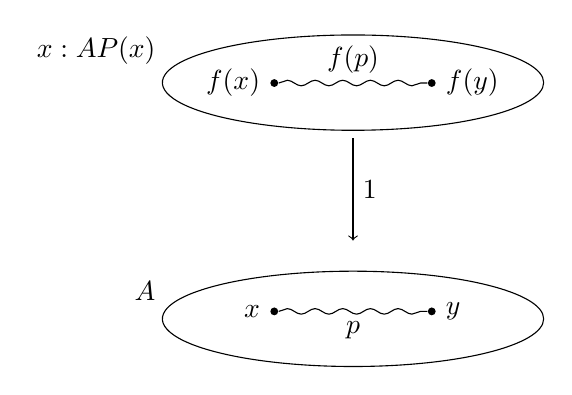
\begin{tikzpicture}[yscale=.5,xscale=2]
    \draw (0,0) arc (-90:170:8ex) node[anchor=south east] {$A$} arc (170:270:8ex);
    \draw (0,6) arc (-90:170:8ex) node[anchor=south east] {$\sm{x:A} P(x)$} arc (170:270:8ex);
    \draw[->] (0,5.8) -- node[auto] {$\proj1$} (0,3.2);
    \node[circle,fill,inner sep=1pt,label=left:{$x$}] (b1) at (-.5,1.4) {};
    \node[circle,fill,inner sep=1pt,label=right:{$y$}] (b2) at (.5,1.4) {};
    \draw[decorate,decoration={snake,amplitude=1}] (b1) -- node[auto,swap] {$p$} (b2);
    \node[circle,fill,inner sep=1pt,label=left:{$f(x)$}] (b1) at (-.5,7.2) {};
    \node[circle,fill,inner sep=1pt,label=right:{$f(y)$}] (b2) at (.5,7.2) {};
    \draw[decorate,decoration={snake,amplitude=1}] (b1) -- node[auto] {$f(p)$} (b2);
  \end{tikzpicture}
\end{center}

We \emph{can} obtain such a thing from \autoref{lem:map}.
Given $f:\prd{x:A} P(x)$, we can define a non-dependent function $f':A\to \sm{x:A} P(x)$ by setting $f'(x)\defeq (x,f(x))$, and then consider $\ap{f'}{p} : f'(x) = f'(y)$.
However, it is not obvious from the type of such a path that it lies over a specific path in $A$ (in this case, $p$), which is sometimes important.

The solution is to use the transport lemma.
Since there is a canonical path from $u:P(x)$ to $\trans p u :P(y)$ which (at least intuitively) lies over $p$, any path from $u$ to $v:P(y)$ lying over $p$ should factor through this path, essentially uniquely, by a path from $\trans p u$ to $v$ lying entirely in the fiber $P(y)$.
Thus, up to equivalence, it makes sense to define ``a path from $u$ to $v$ lying over $p:x=y$'' to mean a path $\trans p u = v$ in $P(y)$.
And, indeed, we can show that dependent functions produce such paths.

\begin{lem}[Dependent map]\label{lem:mapdep}
  \indexdef{application!of dependent function to a path}%
  \indexdef{path!application of a dependent function to}%
  \indexdef{function!dependent!application to a path of}%
  \indexdef{action!of a dependent function on a path}%
  Suppose $f:\prd{x: A} P(x)$; then we have a map
  \[\apdfunc f : \prd{p:x=y}\big(\id[P(y)]{\trans p{f(x)}}{f(y)}\big).\]
\end{lem}

\begin{proof}[First proof]
  Let $D:\prd{x,y:A}{p:\id{x}{y}} \type$ be the type family defined by
  \begin{equation*}
    D(x,y,p)\defeq \trans p {f(x)}= f(y).
  \end{equation*}
  Then $D(x,x,\refl{x})$ is $\trans{(\refl{x})}{f(x)}= f(x)$.
  But since $\trans{(\refl{x})}{f(x)}\jdeq f(x)$, we get that $D(x,x,\refl{x})\jdeq (f(x)= f(x))$.
  Thus, we find the function
  \begin{equation*}
    d\defeq\lam{x} \refl{f(x)}:\prd{x:A} D(x,x,\refl{x})
  \end{equation*}
  and now path induction gives us $\apdfunc f(p):\trans p{f(x)}= f(y)$ for each $p:x= y$.
\end{proof}

\begin{proof}[Second proof]
  By induction, it suffices to assume $p$ is $\refl x$.
  But in this case, the desired equation is $\trans{(\refl{x})}{f(x)}\jdeq f(x)$, which holds judgmentally.
\end{proof}

We will refer generally to paths which ``lie over other paths'' in this sense as \emph{dependent paths}.
\indexsee{dependent!path}{path, dependent}%
\index{path!dependent}%
They will play an increasingly important role starting in \autoref{cha:hits}.
In \autoref{sec:computational} we will see that for a few particular kinds of type families, there are equivalent ways to represent the notion of dependent paths that are sometimes more convenient.

Now recall from \autoref{sec:pi-types} that a non-dependently typed function $f:A\to B$ is just the special case of a dependently typed function $f:\prd{x:A} P(x)$ when $P$ is a constant type family, $P(x) \defeq B$.
In this case, $\apdfunc{f}$ and $\apfunc{f}$ are closely related, because of the following lemma:

\begin{lem}\label{thm:trans-trivial}
  If $P:A\to\type$ is defined by $P(x) \defeq B$ for a fixed $B:\type$, then for any $x,y:A$ and $p:x=y$ and $b:B$ we have a path
  \[ \transconst Bpb : \transfib P p b = b. \]
\end{lem}
\begin{proof}[First proof]
  Fix a $b:B$, and let $D:\prd{x,y:A}{p:\id{x}{y}} \type$ be the type family defined by
  \[ D(x,y,p) \defeq (\transfib P p b = b). \]
  Then $D(x,x,\refl x)$ is $(\transfib P{\refl{x}}{b} = b)$, which is judgmentally equal to $(b=b)$ by the computation rule for transporting.
  Thus, we have the function
  \[ d \defeq \lam{x} \refl{b} : \prd{x:A} D(x,x,\refl x). \]
  Now path induction gives us an element of
  \narrowequation{
    \prd{x,y:A}{p:x=y}(\transfib P p b = b),}
  as desired.
\end{proof}
\begin{proof}[Second proof]
  By induction, it suffices to assume $y$ is $x$ and $p$ is $\refl x$.
  But $\transfib P {\refl x} b \jdeq b$, so in this case what we have to prove is $b=b$, and we have $\refl{b}$ for this.
\end{proof}

Thus, for any $x,y:A$ and $p:x=y$ and $f:A\to B$, by concatenating with $\transconst Bp{f(x)}$ and its inverse, respectively, we obtain functions
\begin{align}
  \big(f(x) = f(y)\big) &\to \big(\trans{p}{f(x)} = f(y)\big)\label{eq:ap-to-apd}
  \qquad\text{and} \\
  \big(\trans{p}{f(x)} = f(y)\big) &\to \big(f(x) = f(y)\big).\label{eq:apd-to-ap}
\end{align}
In fact, these functions are inverse equivalences (in the sense to be introduced in \autoref{sec:basics-equivalences}), and they relate $\apfunc f (p)$  to $\apdfunc f (p)$.

\begin{lem}\label{thm:apd-const}
  For $f:A\to B$ and $p:\id[A]xy$, we have
  \[ \apdfunc f(p) = \transconst B p{f(x)} \ct \apfunc f (p). \]
\end{lem}
\begin{proof}[First proof]
  Let $D:\prd{x,y:A}{p:\id xy} \type$ be the type family defined by
  \[ D(x,y,p) \defeq \big(\apdfunc f (p) = \transconst Bp{f(x)} \ct \apfunc f (p)\big). \]
  Thus, we have
  \[D(x,x,\refl x) \jdeq \big(\apdfunc f (\refl x) = \transconst B{\refl x}{f(x)} \ct \apfunc f ({\refl x})\big).\]
  But by definition, all three paths appearing in this type are $\refl{f(x)}$, so we have
  \[ \refl{\refl{f(x)}} : D(x,x,\refl x). \]
  Thus, path induction gives us an element of $\prd{x,y:A}{p:x=y} D(x,y,p)$, which is what we wanted.
\end{proof}
\begin{proof}[Second proof]
  By induction, it suffices to assume $y$ is $x$ and $p$ is $\refl x$.
  In this case, what we have to prove is $\refl{f(x)} = \refl{f(x)} \ct \refl{f(x)}$, which is true judgmentally.
\end{proof}

Because the types of $\apdfunc{f}$ and $\apfunc{f}$ are different, it is often clearer to use different notations for them.
% We may sometimes use a notation $\apd f p$ for $\apdfunc{f}(p)$, which is similar to the notation $\ap f p$ for $\apfunc{f}(p)$.

\index{function!dependent|)}%

At this point, we hope the reader is starting to get a feel for proofs by induction on identity types.
From now on we stop giving both styles of proofs, allowing ourselves to use whatever is most clear and convenient (and often the second, more concise one).
Here are a few other useful lemmas about transport; we leave it to the reader to give the proofs (in either style).

\begin{lem}\label{thm:transport-concat}
  Given $P:A\to\type$ with $p:\id[A]xy$ and $q:\id[A]yz$ while $u:P(x)$, we have
  \[ \trans{q}{\trans{p}{u}} = \trans{(p\ct q)}{u}. \]
\end{lem}

\begin{lem}\label{thm:transport-compose}
  For a function $f:A\to B$ and a type family $P:B\to\type$, and any $p:\id[A]xy$ and $u:P(f(x))$, we have
  \[ \transfib{P\circ f}{p}{u} = \transfib{P}{\apfunc f(p)}{u}. \]
\end{lem}

\begin{lem}\label{thm:ap-transport}
  For $P,Q:A\to \type$ and a family of functions $f:\prd{x:A} P(x)\to Q(x)$, and any $p:\id[A]xy$ and $u:P(x)$, we have
  \[ \transfib{Q}{p}{f_x(u)} = f_y(\transfib{P}{p}{u}). \]
\end{lem}

\index{type!family of|)}%
\index{transport|)}

\section{Homotopies and equivalences}
\label{sec:basics-equivalences}

\index{homotopy|(defstyle}%

So far, we have seen how the identity type $\id[A]xy$ can be regarded as a type of \emph{identifications}, \emph{paths}, or \emph{equivalences} between two elements $x$ and $y$ of a type $A$.
Now we investigate the appropriate notions of ``identification'' or ``sameness'' between \emph{functions} and between \emph{types}.
In \autoref{sec:compute-pi,sec:compute-universe}, we will see that homotopy type theory allows us to identify these with instances of the identity type, but before we can do that we need to understand them in their own right.

Traditionally, we regard two functions as the same if they take equal values on all inputs.
Under the propositions-as-types interpretation, this suggests that two functions $f$ and $g$ (perhaps dependently typed) should be the same if the type $\prd{x:A} (f(x)=g(x))$ is inhabited.
Under the homotopical interpretation, this dependent function type consists of \emph{continuous} paths or \emph{functorial} equivalences, and thus may be regarded as the type of \emph{homotopies} or of \emph{natural isomorphisms}.\index{isomorphism!natural}%
We will adopt the topological terminology for this.

\begin{defn} \label{defn:homotopy}
  Let $f,g:\prd{x:A} P(x)$ be two sections of a type family $P:A\to\type$.
  A \define{homotopy}
  from $f$ to $g$ is a dependent function of type
  \begin{equation*}
    (f\htpy g) \defeq \prd{x:A} (f(x)=g(x)).
  \end{equation*}
\end{defn}

Note that a homotopy is not the same as an identification $(f=g)$.
However, in \autoref{sec:compute-pi} we will introduce an axiom making homotopies and identifications ``equivalent''.

The following proofs are left to the reader.

\begin{lem}\label{lem:homotopy-props}
  Homotopy is an equivalence relation on each function type $A\to B$.
  That is, we have elements of the types
  \begin{gather*}
    \prd{f:A\to B} (f\htpy f)\\
    \prd{f,g:A\to B} (f\htpy g) \to (g\htpy f)\\
    \prd{f,g,h:A\to B} (f\htpy g) \to (g\htpy h) \to (f\htpy h).
  \end{gather*}
\end{lem}

% This is judgmental and is \autoref{ex:composition}.
% \begin{lem}
%   Composition is associative and unital up to homotopy.
%   That is:
%   \begin{enumerate}
%   \item If $f:A\to B$ then $f\circ \idfunc[A]\htpy f\htpy \idfunc[B]\circ f$.
%   \item If $f:A\to B, g:B\to C$ and $h:C\to D$ then $h\circ (g\circ f) \htpy (h\circ g)\circ f$.
%   \end{enumerate}
% \end{lem}

\index{functoriality of functions in type theory@``functoriality'' of functions in type theory}%
\index{continuity of functions in type theory@``continuity'' of functions in type theory}%
Just as functions in type theory are automatically ``functors'', homotopies are automatically
\index{naturality of homotopies@``naturality'' of homotopies}%
``natural transformations'', in the following sense.
Recall that for $f:A\to B$ and $p:\id[A]xy$, we may write $\ap f p$ to mean $\apfunc{f} (p)$.

\begin{lem}\label{lem:htpy-natural}
  Suppose $H:f\htpy g$ is a homotopy between functions $f,g:A\to B$ and let $p:\id[A]xy$.  Then we have
  \begin{equation*}
    H(x)\ct\ap{g}{p}=\ap{f}{p}\ct H(y).
  \end{equation*}
  We may also draw this as a commutative diagram:\index{diagram}
  \begin{align*}
    \xymatrix{
      f(x) \ar@{=}[r]^{\ap fp} \ar@{=}[d]_{H(x)} & f(y) \ar@{=}[d]^{H(y)} \\
      g(x) \ar@{=}[r]_{\ap gp} & g(y)
    }
  \end{align*}
\end{lem}
\begin{proof}
  By induction, we may assume $p$ is $\refl x$.
  Since $\apfunc{f}$ and $\apfunc g$ compute on reflexivity, in this case what we must show is
  \[ H(x) \ct \refl{g(x)} = \refl{f(x)} \ct H(x). \]
  But this follows since both sides are equal to $H(x)$.
\end{proof}

\begin{cor}\label{cor:hom-fg}
  Let $H : f \htpy \idfunc[A]$ be a homotopy, with $f : A \to A$. Then for any $x : A$ we have \[ H(f(x)) = \ap f{H(x)}. \]
  % The above path will be denoted by $\com{H}{f}{x}$.
\end{cor}
\noindent
Here $f(x)$ denotes the ordinary application of $f$ to $x$, while $\ap f{H(x)}$ denotes $\apfunc{f}(H(x))$.
\begin{proof}
By naturality of $H$, the following diagram of paths commutes:
\begin{align*}
\xymatrix@C=3pc{
ffx \ar@{=}[r]^-{\ap f{Hx}} \ar@{=}[d]_{H(fx)} & fx \ar@{=}[d]^{Hx} \\
fx \ar@{=}[r]_-{Hx} & x
}
\end{align*}
That is, $\ap f{H x} \ct H x = H(f x) \ct H x$.
We can now whisker by $\opp{(H x)}$ to cancel $H x$, obtaining
\[ \ap f{H x}
= \ap f{H x} \ct H x \ct \opp{(H x)}
= H(f x) \ct H x \ct \opp{(H x)}
= H(f x)
\]
as desired (with some associativity paths suppressed).
\end{proof}

Of course, like the functoriality of functions (\autoref{lem:ap-functor}), the equality in \autoref{lem:htpy-natural} is a path which satisfies its own coherence laws, and so on.

\index{homotopy|)}%

\index{equivalence|(}%
Moving on to types, from a traditional perspective one may say that a function $f:A\to B$ is an \emph{isomorphism} if there is a function $g:B\to A$ such that both composites $f\circ g$ and $g\circ f$ are pointwise equal to the identity, i.e.\ such that $f \circ g \htpy \idfunc[B]$ and $g\circ f \htpy \idfunc[A]$.
\indexsee{homotopy!equivalence}{equivalence}%
A homotopical perspective suggests that this should be called a \emph{homotopy equivalence}, and from a categorical one, it should be called an \emph{equivalence of (higher) groupoids}.
However, when doing proof-relevant mathematics,
\index{mathematics!proof-relevant}%
the corresponding type
\begin{equation}
  \sm{g:B\to A} \big((f \circ g \htpy \idfunc[B]) \times (g\circ f \htpy \idfunc[A])\big)\label{eq:qinvtype}
\end{equation}
is poorly behaved.
For instance, for a single function $f:A\to B$ there may be multiple unequal inhabitants of~\eqref{eq:qinvtype}.
(This is closely related to the observation in higher category theory that often one needs to consider \emph{adjoint} equivalences\index{adjoint!equivalence} rather than plain equivalences.)
For this reason, we give~\eqref{eq:qinvtype} the following historically accurate, but slightly de\-rog\-a\-to\-ry-sounding name instead.

\begin{defn}\label{defn:quasi-inverse}
  For a function $f:A\to B$, a \define{quasi-inverse}
  \indexdef{quasi-inverse}%
  \indexsee{function!quasi-inverse of}{quasi-inverse}%
  of $f$ is a triple $(g,\alpha,\beta)$ consisting of a function $g:B\to A$ and homotopies
$\alpha:f\circ g\htpy \idfunc[B]$ and $\beta:g\circ f\htpy \idfunc[A]$.
\end{defn}

\symlabel{qinv}
Thus,~\eqref{eq:qinvtype} is \emph{the type of quasi-inverses of $f$}; we may denote it by $\qinv(f)$.

\begin{eg}\label{eg:idequiv}
  \index{identity!function}%
  \index{function!identity}%
  The identity function $\idfunc[A]:A\to A$ has a quasi-inverse given by $\idfunc[A]$ itself, together with homotopies defined by $\alpha(y) \defeq \refl{y}$ and $\beta(x) \defeq \refl{x}$.
\end{eg}

\begin{eg}\label{eg:concatequiv}
  For any $p:\id[A]xy$ and $z:A$, the functions
  \begin{align*}
    (p\ct \blank)&:(\id[A]yz) \to (\id[A]xz) \qquad\text{and}\\
    (\blank \ct p)&:(\id[A]zx) \to (\id[A]zy)
  \end{align*}
  have quasi-inverses given by $(\opp p \ct \blank)$ and $(\blank \ct \opp p)$, respectively; see \autoref{ex:equiv-concat}.
\end{eg}

\begin{eg}\label{thm:transportequiv}
  For any $p:\id[A]xy$ and $P:A\to\type$, the function
  \[\transfib{P}{p}{\blank}:P(x) \to P(y)\]
  has a quasi-inverse given by $\transfib{P}{\opp p}{\blank}$; this follows from \autoref{thm:transport-concat}.
\end{eg}

\symlabel{basics-isequiv}
In general, we will only use the word \emph{isomorphism}
\index{isomorphism!of sets}
(and similar words such as \emph{bijection})
\index{bijection}
in the special case when the types $A$ and $B$ ``behave like sets'' (see \autoref{sec:basics-sets}).
In this case, the type~\eqref{eq:qinvtype} is unproblematic.
We will reserve the word \emph{equivalence} for an improved notion $\isequiv (f)$ with the following properties:%
\begin{enumerate}
\item For each $f:A\to B$ there is a function $\qinv(f) \to \isequiv (f)$.\label{item:be1}
\item Similarly, for each $f$ we have $\isequiv (f) \to \qinv(f)$; thus the two are logically equivalent (see \autoref{sec:pat}).\label{item:be2}
\item For any two inhabitants $e_1,e_2:\isequiv(f)$ we have $e_1=e_2$.\label{item:be3}
\end{enumerate}
In \autoref{cha:equivalences} we will see that there are many different definitions of $\isequiv(f)$ which satisfy these three properties, but that all of them are equivalent.
For now, to convince the reader that such things exist, we mention only the easiest such definition:
\begin{equation}\label{eq:isequiv-invertible}
  \isequiv(f) \;\defeq\;
  \Parens{\sm{g:B\to A} (f\circ g \htpy \idfunc[B])}
  \times
  \Parens{\sm{h:B\to A} (h\circ f \htpy \idfunc[A])}.
\end{equation}
We can show~\ref{item:be1} and~\ref{item:be2} for this definition now.
A function $\qinv(f) \to \isequiv (f)$ is easy to define by taking $(g,\alpha,\beta)$ to $(g,\alpha,g,\beta)$.
In the other direction, given $(g,\alpha,h,\beta)$, let $\gamma$ be the composite homotopy
\[ g \overset{\beta}{\htpy} h\circ f\circ g \overset{\alpha}{\htpy} h \]
and let $\beta':g\circ f\htpy \idfunc[A]$ be obtained from $\gamma$ and $\beta$.
Then $(g,\alpha,\beta'):\qinv(f)$.

Property~\ref{item:be3} for this definition is not too hard to prove either, but it requires identifying the identity types of cartesian products and dependent pair types, which we will discuss in \autoref{sec:compute-cartprod,sec:compute-sigma}.
Thus, we postpone it as well; see \autoref{sec:biinv}.
At this point, the main thing to take away is that there is a well-behaved type which we can pronounce as ``$f$ is an equivalence'', and that we can prove $f$ to be an equivalence by exhibiting a quasi-inverse to it.
In practice, this is the most common way to prove that a function is an equivalence.

In accord with the proof-relevant philosophy,
\index{mathematics!proof-relevant}%
\emph{an equivalence} from $A$ to $B$ is defined to be a function $f:A\to B$ together with an inhabitant of $\isequiv (f)$, i.e.\ a proof that it is an equivalence.
We write $(\eqv A B)$ for the type of equivalences from $A$ to $B$, i.e.\ the type
\begin{equation}\label{eq:eqv}
  (\eqv A B) \defeq \sm{f:A\to B} \isequiv(f).
\end{equation}
Property~\ref{item:be3} above will ensure that if two equivalences are equal as functions (that is, the underlying elements of $A\to B$ are equal), then they are also equal as equivalences (see \autoref{sec:compute-sigma}).
Thus, we often abuse notation by denoting an equivalence by the same letter as its underlying function.

We conclude by observing:

\begin{lem}\label{thm:equiv-eqrel}
  Type equivalence is an equivalence relation on \type.
  More specifically:
  \begin{enumerate}
  \item For any $A$, the identity function $\idfunc[A]$ is an equivalence; hence $\eqv A A$.
  \item For any $f:\eqv A B$, we have an equivalence $f^{-1} : \eqv B A$.
  \item For any $f:\eqv A B$ and $g:\eqv B C$, we have $g\circ f : \eqv A C$.
  \end{enumerate}
\end{lem}
\begin{proof}
  The identity function is clearly its own quasi-inverse; hence it is an equivalence.

  If $f:A\to B$ is an equivalence, then it has a quasi-inverse, say $f^{-1}:B\to A$.
  Then $f$ is also a quasi-inverse of $f^{-1}$, so $f^{-1}$ is an equivalence $B\to A$.

  Finally, given $f:\eqv A B$ and $g:\eqv B C$ with quasi-inverses $f^{-1}$ and $g^{-1}$, say, then for any $a:A$ we have $f^{-1} g^{-1} g f a = f^{-1} f a = a$, and for any $c:C$ we have $g f f^{-1} g^{-1} c = g g^{-1} c = c$.
  Thus $f^{-1} \circ g^{-1}$ is a quasi-inverse to $g\circ f$, hence the latter is an equivalence.
\end{proof}

\index{equivalence|)}%


\section{The higher groupoid structure of type formers}
\label{sec:computational}

In \autoref{cha:typetheory}, we introduced many ways to form new types: cartesian products, disjoint unions, dependent products, dependent sums, etc.
In \autoref{sec:equality,sec:functors,sec:fibrations}, we saw that \emph{all} types in homotopy type theory behave like spaces or higher groupoids.
Our goal in the rest of the chapter is to make explicit how this higher structure behaves in the case of the particular types defined in \autoref{cha:typetheory}.

It turns out that for many types $A$, the equality types $\id[A]xy$ can be characterized, up to equivalence, in terms of whatever data was used to construct $A$.
For example, if $A$ is a cartesian product $B\times C$, and $x\jdeq (b,c)$ and $y\jdeq(b',c')$, then we have an equivalence
\begin{equation}\label{eq:prodeqv}
  \eqv{\big((b,c)=(b',c')\big)}{\big((b=b')\times (c=c')\big)}.
\end{equation}
In more traditional language, two ordered pairs are equal just when their components are equal (but the equivalence~\eqref{eq:prodeqv} says rather more than this).
The higher structure of the identity types can also be expressed in terms of these equivalences; for instance, concatenating two equalities between pairs corresponds to pairwise concatenation.

Similarly, when a type family $P:A\to\type$ is built up fiberwise using the type forming rules from \autoref{cha:typetheory}, the operation $\transfib{P}{p}{\blank}$ can be characterized, up to homotopy, in terms of the corresponding operations on the data that went into $P$.
For instance, if $P(x) \jdeq B(x)\times C(x)$, then we have
\[\transfib{P}{p}{(b,c)} = \big(\transfib{B}{p}{b},\transfib{C}{p}{c}\big).\]

Finally, the type forming rules are also functorial, and if a function $f$ is built from this functoriality, then the operations $\apfunc f$ and $\apdfunc f$ can be computed based on the corresponding ones on the data going into $f$.
For instance, if $g:B\to B'$ and $h:C\to C'$ and we define $f:B\times C \to B'\times C'$ by $f(b,c)\defeq (g(b),h(c))$, then modulo the equivalence~\eqref{eq:prodeqv}, we can identify $\apfunc f$ with ``$(\apfunc g,\apfunc h)$''.

The next few sections (\crefrange{sec:compute-cartprod}{sec:compute-nat}) will be devoted to stating and proving theorems of this sort for all the basic type forming rules, with one section for each basic type former.
Here we encounter a certain apparent deficiency in currently available type theories;
as will become clear in later chapters, it would seem to be more convenient and intuitive if these characterizations of identity types, transport, and so on were \emph{judgmental}\index{judgmental equality} equalities.
However, in the theory presented in \autoref{cha:typetheory}, the identity types are defined uniformly for all types by their induction principle, so we cannot ``redefine'' them to be different things at different types.
Thus, the characterizations for particular types to be discussed in this chapter are, for the most part, \emph{theorems} which we have to discover and prove, if possible.

Actually, the type theory of \autoref{cha:typetheory} is insufficient to prove the desired theorems for two of the type formers: $\Pi$-types and universes.
For this reason, we are forced to introduce axioms into our type theory, in order to make those ``theorems'' true.
Type-theoretically, an \emph{axiom} (c.f.~\autoref{sec:axioms}) is an ``atomic'' element that is declared to inhabit some specified type, without there being any rules governing its behavior other than those pertaining to the type it inhabits.
\index{axiom!versus rules}%

\index{function extensionality}%
\indexsee{extensionality, of functions}{function extensionality}
\index{univalence axiom}%
The axiom for $\Pi$-types (\autoref{sec:compute-pi}) is familiar to type theorists: it is called \emph{function extensionality}, and states (roughly) that if two functions are homotopic in the sense of \autoref{sec:basics-equivalences}, then they are equal.
The axiom for universes (\autoref{sec:compute-universe}), however, is a new contribution of homotopy type theory due to Voevodsky: it is called the \emph{univalence axiom}, and states (roughly) that if two types are equivalent in the sense of \autoref{sec:basics-equivalences}, then they are equal.
We have already remarked on this axiom in the introduction; it will play a very important role in this book.%
\footnote{We have chosen to introduce these principles as axioms, but there are potentially other ways to formulate a type theory in which they hold.
  See the Notes to this chapter.}

It is important to note that not \emph{all} identity types can be ``determined'' by induction over the construction of types.
Counterexamples include most nontrivial higher inductive types (see \autoref{cha:hits,cha:homotopy}).
For instance, calculating the identity types of the types $\Sn^n$ (see \autoref{sec:circle}) is equivalent to calculating the higher homotopy groups of spheres, a deep and important field of research in algebraic topology.


\section{Cartesian product types}
\label{sec:compute-cartprod}

\index{type!product|(}%
Given types $A$ and $B$, consider the cartesian product type $A \times B$.  
For any elements $x,y:A\times B$ and a path $p:\id[A\times B]{x}{y}$, by functoriality we can extract paths $\ap{\proj1}p:\id[A]{\proj1(x)}{\proj1(y)}$ and $\ap{\proj2}p:\id[B]{\proj2(x)}{\proj2(y)}$.
Thus, we have a function
\begin{equation}\label{eq:path-prod}
  (\id[A\times B]{x}{y}) \to (\id[A]{\proj1(x)}{\proj1(y)}) \times (\id[B]{\proj2(x)}{\proj2(y)}).
\end{equation}

\begin{thm}\label{thm:path-prod}
  For any $x$ and $y$, the function~\eqref{eq:path-prod} is an equivalence.
\end{thm}

Read logically, this says that two pairs are equal if they are equal
componentwise.  Read category-theoretically, this says that the
morphisms in a product groupoid are pairs of morphisms.  Read
homotopy-theoretically, this says that the paths in a product
space are pairs of paths.

\begin{proof}
  We need a function in the other direction:
  \begin{equation}
    (\id[A]{\proj1(x)}{\proj1(y)}) \times (\id[B]{\proj2(x)}{\proj2(y)}) \to (\id[A\times B]{x}{y}). \label{eq:path-prod-inverse}
  \end{equation}
  By the induction rule for cartesian products, we may assume that $x$ and $y$ are both pairs, i.e.\ $x\jdeq (a,b)$ and $y\jdeq (a',b')$ for some $a,a':A$ and $b,b':B$.
  In this case, what we want is a function
  \begin{equation*}
    (\id[A]{a}{a'}) \times (\id[B]{b}{b'}) \to \big(\id[A\times B]{(a,b)}{(a',b')}\big).
  \end{equation*}
  Now by induction for the cartesian product in its domain, we may assume given $p:a=a'$ and $q:b=b'$.
  And by two path inductions, we may assume that $a\jdeq a'$ and $b\jdeq b'$ and both $p$ and $q$ are reflexivity.
  But in this case, we have $(a,b)\jdeq(a',b')$ and so we can take the output to also be reflexivity.

  It remains to prove that~\eqref{eq:path-prod-inverse} is quasi-inverse to~\eqref{eq:path-prod}.
  This is a simple sequence of inductions, but they have to be done in the right order.

  In one direction, let us start with $r:\id[A\times B]{x}{y}$.
  We first do a path induction on $r$ in order to assume that $x\jdeq y$ and $r$ is reflexivity.
  In this case, since $\apfunc{\proj1}$ and $\apfunc{\proj2}$ are defined by path induction,~\eqref{eq:path-prod} takes $r\jdeq \refl{x}$ to the pair $(\refl{\proj1x},\refl{\proj2x})$.
  Now by induction on $x$, we may assume $x\jdeq (a,b)$, so that this is $(\refl a, \refl b)$.
  Thus,~\eqref{eq:path-prod-inverse} takes it by definition to $\refl{(a,b)}$, which (under our current assumptions) is $r$.
  
  In the other direction, if we start with $s:(\id[A]{\proj1(x)}{\proj1(y)}) \times (\id[B]{\proj2(x)}{\proj2(y)})$, then we first do induction on $x$ and $y$ to assume that they are pairs $(a,b)$ and $(a',b')$, and then induction on $s:(\id[A]{a}{a'}) \times (\id[B]{b}{b'})$ to reduce it to a pair $(p,q)$ where $p:a=a'$ and $q:b=b'$.
  Now by induction on $p$ and $q$, we may assume they are reflexivities $\refl a$ and $\refl b$, in which case~\eqref{eq:path-prod-inverse} yields $\refl{(a,b)}$ and then~\eqref{eq:path-prod} returns us to $(\refl a,\refl b)\jdeq (p,q)\jdeq s$.
\end{proof}

In particular, we have shown that~\eqref{eq:path-prod} has an inverse~\eqref{eq:path-prod-inverse}, which we may denote by
\symlabel{defn:pairpath}
\[
\pairpath : (\id{\proj{1}(x)}{\proj{1}(y)}) \times (\id{\proj{2}(x)}{\proj{2}(y)}) \to (\id x y).
\]
Note that a special case of this yields the propositional uniqueness principle\index{uniqueness!principle, propositional!for product types} for products: $z = (\proj1(z),\proj2(z))$.

It can be helpful to view \pairpath as a \emph{constructor} or \emph{introduction rule} for $\id x y$, analogous to the ``pairing'' constructor of $A\times B$ itself, which introduces the pair $(a,b)$ given $a:A$ and $b:B$.
From this perspective, the two components of~\eqref{eq:path-prod}:
\begin{align*}
  \projpath{1} &: (\id{x}{y}) \to (\id{\proj{1}(x)}{\proj{1} (y)})\\
  \projpath{2} &: (\id{x}{y}) \to (\id{\proj{2}(x)}{\proj{2} (y)})
\end{align*}
are \emph{elimination} rules.
Similarly, the two homotopies which witness~\eqref{eq:path-prod-inverse} as quasi-inverse to~\eqref{eq:path-prod} consist, respectively, of \emph{propositional computation rules}:
\index{computation rule!propositional!for identities between pairs}%
\begin{align*}
  {\projpath{1}{(\pairpath(p, q)})}
  &= %_{(\id{\proj{1} x}{\proj{1} y})}
  {p} \qquad\text{for } p:\id{\proj{1} x}{\proj{1} y} \\
  {\projpath{2}{(\pairpath(p,q)})}
  &= %_{(\id{\proj{2} x}{\proj{2} y})}
  {q} \qquad\text{for } q:\id{\proj{2} x}{\proj{2} y}
\end{align*}
and a \emph{propositional uniqueness principle}:
\index{uniqueness!principle, propositional!for identities between pairs}%
\[
\id{r}{\pairpath(\projpath{1} (r), \projpath{2} (r)) }
\qquad\text{for } r : \id[A \times B] x y.
\]

We can also characterize the reflexivity, inverses, and composition of paths in $A\times B$ componentwise:
\begin{align*}
  {\refl{(z : A \times B)}}
  &= {\pairpath (\refl{\proj{1} z},\refl{\proj{2} z})} \\
  {\opp{p}}
  &= {\pairpath \big(\opp{\projpath{1} (p)},\, \opp{\projpath{2} (p)}\big)} \\
  {{p \ct q}}
  &= {\pairpath \big({\projpath{1} (p)} \ct {\projpath{1} (q)},\,{\projpath{2} (p)} \ct {\projpath{2} (q)}\big)}.
\end{align*}
The same is true for the rest of the higher groupoid structure considered in \autoref{sec:equality}.
All of these equations can be derived by using path induction on the given paths and then returning reflexivity.  

\index{transport!in product types}%
We now consider transport in a pointwise product of type families.
Given type families $ A, B : Z \to \type$, we abusively write $A\times B:Z\to \type$ for the type family defined by $(A\times B)(z) \defeq A(z) \times B(z)$.
Now given $p : \id[Z]{z}{w}$ and $x : A(z) \times B(z)$, we can transport $x$ along $p$ to obtain an element of $A(w)\times B(w)$.

\begin{thm}\label{thm:trans-prod}
  In the above situation, we have
  \[
  \id[A(w) \times B(w)]
  {\transfib{A\times B}px}
  {(\transfib{A}{p}{\proj{1}x}, \transfib{B}{p}{\proj{2}x})}.
  \]
\end{thm}
\begin{proof}
  By path induction, we may assume $p$ is reflexivity, in which case we have
  \begin{align*}
    \transfib{A\times B}px&\jdeq x\\
    \transfib{A}{p}{\proj{1}x}&\jdeq \proj1x\\
    \transfib{B}{p}{\proj{2}x}&\jdeq \proj2x.
  \end{align*}
  Thus, it remains to show $x = (\proj1 x, \proj2x)$.
  But this is the propositional uniqueness principle for product types, which, as we remarked above, follows from \autoref{thm:path-prod}.
\end{proof}

Finally, we consider the functoriality of $\apfunc{}$ under cartesian products.
Suppose given types $A,B,A',B'$ and functions $g:A\to A'$ and $h:B\to B'$; then we can define a function $f:A\times B\to A'\times B'$ by $f(x) \defeq (g(\proj1x),h(\proj2x))$.

\begin{thm}\label{thm:ap-prod}
  In the above situation, given $x,y:A\times B$ and $p:\proj1x=\proj1y$ and $q:\proj2x=\proj2y$, we have
  \[ \id[(f(x)=f(y))]{\ap{f}{\pairpath(p,q)}} {\pairpath(\ap{g}{p},\ap{h}{q})}. \]
\end{thm}
\begin{proof}
  Note first that the above equation is well-typed.
  On the one hand, since $\pairpath(p,q):x=y$ we have $\ap{f}{\pairpath(p,q)}:f(x)=f(y)$.
  On the other hand, since $\proj1(f(x))\jdeq g(\proj1x)$ and $\proj2(f(x))\jdeq h(\proj2x)$, we also have $\pairpath(\ap{g}{p},\ap{h}{q}):f(x)=f(y)$.

  Now, by induction, we may assume $x\jdeq(a,b)$ and $y\jdeq(a',b')$, in which case we have $p:a=a'$ and $q:b=b'$.
  Thus, by path induction, we may assume $p$ and $q$ are reflexivity, in which case the desired equation holds judgmentally.
\end{proof}

\index{type!product|)}%

\section{\texorpdfstring{$\Sigma$}{Σ}-types}
\label{sec:compute-sigma}

\index{type!dependent pair|(}%
Let $A$ be a type and $B:A\to\type$ a type family.
Recall that the $\Sigma$-type, or dependent pair type, $\sm{x:A} B(x)$ is a generalization of the cartesian product type.
Thus, we expect its higher groupoid structure to also be a generalization of the previous section.
In particular, its paths should be pairs of paths, but it takes a little thought to give the correct types of these paths.

Suppose that we have a path $p:w=w'$ in $\sm{x:A}P(x)$.
Then we get $\ap{\proj{1}}{p}:\proj{1}(w)=\proj{1}(w')$.
However, we cannot directly ask whether $\proj{2}(w)$ is identical to $\proj{2}(w')$ since they don't have to be in the same type.
But we can transport\index{transport} $\proj{2}(w)$ along the path $\ap{\proj{1}}{p}$, and this does give us an element of the same type as $\proj{2}(w')$.
By path induction, we do in fact obtain a path $\trans{\ap{\proj{1}}{p}}{\proj{2}(w)}=\proj{2}(w')$.

Recall from the discussion preceding \autoref{lem:mapdep} that
\narrowequation{
  \trans{\ap{\proj{1}}{p}}{\proj{2}(w)}=\proj{2}(w')
}
can be regarded as the type of paths from $\proj2(w)$ to $\proj2(w')$ which lie over the path $\ap{\proj1}{p}$ in $A$.
\index{fibration}%
\index{total!space}%
Thus, we are saying that a path $w=w'$ in the total space determines (and is determined by) a path $p:\proj1(w)=\proj1(w')$ in $A$ together with a path from $\proj2(w)$ to $\proj2(w')$ lying over $p$, which seems sensible.

\begin{rmk}
  Note that if we have $x:A$ and $u,v:P(x)$ such that $(x,u)=(x,v)$, it does not follow that $u=v$.
  All we can conclude is that there exists $p:x=x$ such that $\trans p u = v$.
  This is a well-known source of confusion for newcomers to type theory, but it makes sense from a topological viewpoint: the existence of a path $(x,u)=(x,v)$ in the total space of a fibration between two points that happen to lie in the same fiber does not imply the existence of a path $u=v$ lying entirely \emph{within} that fiber.
\end{rmk}

The next theorem states that we can also reverse this process.
Since it is a direct generalization of \autoref{thm:path-prod}, we will be more concise.

\begin{thm}\label{thm:path-sigma}
Suppose that $P:A\to\type$ is a type family over a type $A$ and let $w,w':\sm{x:A}P(x)$. Then there is an equivalence
\begin{equation*}
\eqvspaced{(w=w')}{\dsm{p:\proj{1}(w)=\proj{1}(w')} \trans{p}{\proj{2}(w)}=\proj{2}(w')}.
\end{equation*}
\end{thm}

\begin{proof}
We define for any $w,w':\sm{x:A}P(x)$, a function
\begin{equation*}
f: (w=w') \to \dsm{p:\proj{1}(w)=\proj{1}(w')} \trans{p}{\proj{2}(w)}=\proj{2}(w')
\end{equation*}
by path induction, with
\begin{equation*}
f(w,w,\refl{w})\defeq(\refl{\proj{1}(w)},\refl{\proj{2}(w)}).
\end{equation*}
We want to show that $f$ is an equivalence.

In the reverse direction, we define
\begin{narrowmultline*}
  g : \prd{w,w':\sm{x:A}P(x)} 
      \Parens{\sm{p:\proj{1}(w)=\proj{1}(w')}\trans{p}{\proj{2}(w)}=\proj{2}(w')}
      \to
      \narrowbreak
      (w=w')
\end{narrowmultline*}
by first inducting on $w$ and $w'$, which splits them into $(w_1,w_2)$ and
$(w_1',w_2')$ respectively, so it suffices to show 
\begin{equation*}
\Parens{\sm{p:w_1 = w_1'}\trans{p}{w_2}=w_2'} \to ((w_1,w_2)=(w_1',w_2')).
\end{equation*}
Next, given a pair $\sm{p:w_1 = w_1'}\trans{p}{w_2}=w_2'$, we can
use $\Sigma$-induction to get $p : w_1 = w_1'$ and $q :
\trans{p}{w_2}=w_2'$.  Inducting on $p$, we have $q :
\trans{\refl{}}{w_2}=w_2'$, and it suffices to show 
$(w_1,w_2)=(w_1,w_2')$.  But $\trans{\refl{}}{w_2} \jdeq w_2$, so
inducting on $q$ reduces to the goal to 
$(w_1,w_2)=(w_1,w_2)$, which we can prove with $\refl{(w_1,w_2)}$.  

Next we show that $f \circ g$ is the identity for all $w$, $w'$ and
$r$, where $r$ has type
\[\dsm{p:\proj{1}(w)=\proj{1}(w')} (\trans{p}{\proj{2}(w)}=\proj{2}(w')).\]
First, we break apart the pairs $w$, $w'$, and $r$ by pair induction, as in the
definition of $g$, and then use two path inductions to reduce both components
of $r$ to \refl{}.  Then it suffices to show that 
$f (g(\refl{},\refl{})) = \refl{}$, which is true by definition.

Similarly, to show that $g \circ f$ is the identity for all $w$, $w'$,
and $p : w = w'$, we can do path induction on $p$, and then induction to
split $w$, at which point it suffices to show that
$g(f (\refl{(w_1,w_2)})) = \refl{(w_1,w_2)}$, which is true by
definition.

Thus, $f$ has a quasi-inverse, and is therefore an equivalence.  
\end{proof}

As we did in the case of cartesian products, we can deduce a propositional uniqueness principle as a special case.

\begin{cor}\label{thm:eta-sigma}
  \index{uniqueness!principle, propositional!for dependent pair types}%
  For $z:\sm{x:A} P(x)$, we have $z = (\proj1(z),\proj2(z))$.
\end{cor}
\begin{proof}
  We have $\refl{\proj1(z)} : \proj1(z) = \proj1(\proj1(z),\proj2(z))$, so by \autoref{thm:path-sigma} it will suffice to exhibit a path $\trans{(\refl{\proj1(z)})}{\proj2(z)} = \proj2(\proj1(z),\proj2(z))$.
  But both sides are judgmentally equal to $\proj2(z)$.
\end{proof}

Like with binary cartesian products, we can think of 
the backward direction of \autoref{thm:path-sigma} as
an introduction form (\pairpath{}{}), the forward direction as
elimination forms (\projpath{1} and \projpath{2}), and the equivalence
as giving a propositional computation rule and uniqueness principle for these.

Note that the lifted path $\mathsf{lift}(u,p)$  of $p:x=y$ at $u:P(x)$ defined in \autoref{thm:path-lifting} may be identified with the special case of the introduction form
\[\pairpath(p,\refl{\trans p u}):(x,u) = (y,\trans p u).\]
\index{transport!in dependent pair types}%
This appears in the statement of action of transport on $\Sigma$-types, which is also a generalization of the action for binary cartesian products:

\begin{thm}\label{transport-Sigma}
  Suppose we have type families
  %
  \begin{equation*}
    P:A\to\type
    \qquad\text{and}\qquad
    Q:\Parens{\sm{x:A} P(x)}\to\type.
  \end{equation*}
  %
  Then we can construct the type family over $A$ defined by
  \begin{equation*}
    x \mapsto \sm{u:P(x)} Q(x,u).
  \end{equation*}
  For any path $p:x=y$ and any $(u,z):\sm{u:P(x)} Q(x,u)$ we have
  \begin{equation*}
    \trans{p}{u,z}=\big(\trans{p}{u},\,\trans{\pairpath(p,\refl{\trans pu})}{z}\big).
  \end{equation*}
\end{thm}

\begin{proof}
Immediate by path induction.
\end{proof}

We leave it to the reader to state and prove a generalization of
\autoref{thm:ap-prod} (see \autoref{ex:ap-sigma}), and to characterize
the reflexivity, inverses, and composition of $\Sigma$-types
componentwise.

\index{type!dependent pair|)}%

\section{The unit type}
\label{sec:compute-unit}

\index{type!unit|(}%
Trivial cases are sometimes important, so we mention briefly the case of the unit type~\unit.

\begin{thm}\label{thm:path-unit}
  For any $x,y:\unit$, we have $\eqv{(x=y)}{\unit}$.
\end{thm}
\begin{proof}
  A function $(x=y)\to\unit$ is easy to define by sending everything to \ttt.
  Conversely, for any $x,y:\unit$ we may assume by induction that $x\jdeq \ttt\jdeq y$.
  In this case we have $\refl{\ttt}:x=y$, yielding a constant function $\unit\to(x=y)$.

  To show that these are inverses, consider first an element $u:\unit$.
  We may assume that $u\jdeq\ttt$, but this is also the result of the composite $\unit \to (x=y)\to\unit$.

  On the other hand, suppose given $p:x=y$.
  By path induction, we may assume $x\jdeq y$ and $p$ is $\refl x$.
  We may then assume that $x$ is \ttt, in which case the composite $(x=y) \to \unit\to(x=y)$ takes $p$ to $\refl x$, i.e.\ to~$p$.
\end{proof}

In particular, any two elements of $\unit$ are equal.
We leave it to the reader to formulate this equivalence in terms of introduction, elimination, computation, and uniqueness rules.
\index{transport!in unit type}%
The transport lemma for \unit is simply the transport lemma for constant type families (\autoref{thm:trans-trivial}).

\index{type!unit|)}%

\section{\texorpdfstring{$\Pi$}{Π}-types and the function extensionality axiom}
\label{sec:compute-pi}

\index{type!dependent function|(}%
\index{type!function|(}%
\index{homotopy|(}%
Given a type $A$ and a type family $B : A \to \type$, consider the dependent function type $\prd{x:A}B(x)$.
We expect the type $f=g$ of paths from $f$ to $g$ in $\prd{x:A} B(x)$ to be equivalent to 
the type of pointwise paths:\index{pointwise!equality of functions}
\begin{equation}
  \eqvspaced{(\id{f}{g})}{\Parens{\prd{x:A} (\id[B(x)]{f(x)}{g(x)})}}.\label{eq:path-forall}
\end{equation}
From a traditional perspective, this would say that two functions which are equal at each point are equal as functions.
\index{continuity of functions in type theory@``continuity'' of functions in type theory}%
From a topological perspective, it would say that a path in a function space is the same as a continuous homotopy.
\index{functoriality of functions in type theory@``functoriality'' of functions in type theory}%
And from a categorical perspective, it would say that an isomorphism in a functor category is a natural family of isomorphisms.

Unlike the case in the previous sections, however, the basic type theory presented in \autoref{cha:typetheory} is insufficient to prove~\eqref{eq:path-forall}.
All we can say is that there is a certain function
\begin{equation}\label{eq:happly}
  \happly : (\id{f}{g}) \to \prd{x:A} (\id[B(x)]{f(x)}{g(x)})
\end{equation}
which is easily defined by path induction.
For the moment, therefore, we will assume:

\begin{axiom}[Function extensionality]\label{axiom:funext}
  \indexsee{axiom!function extensionality}{function extensionality}%
  \indexdef{function extensionality}%
  For any $A$, $B$, $f$, and $g$, the function~\eqref{eq:happly} is an equivalence.
\end{axiom}

We will see in later chapters that this axiom follows both from univalence (see \autoref{sec:compute-universe,sec:univalence-implies-funext}) and from an interval type (see \autoref{sec:interval} and \autoref{ex:funext-from-interval}).

In particular, \autoref{axiom:funext} implies that~\eqref{eq:happly} has a quasi-inverse
\[
\funext : \Parens{\prd{x:A} (\id{f(x)}{g(x)})} \to {(\id{f}{g})}.
\]
This function is also referred to as ``function extensionality''.
As we did with $\pairpath$ in \autoref{sec:compute-cartprod}, we can regard $\funext$ as an \emph{introduction rule} for the type $\id f g$.
From this point of view, $\happly$ is the \emph{elimination rule}, while the homotopies witnessing $\funext$ as quasi-inverse to $\happly$ become a propositional computation rule\index{computation rule!propositional!for identities between functions}
\[
\id{\happly({\funext{(h)}},x)}{h(x)} \qquad\text{for }h:\prd{x:A} (\id{f(x)}{g(x)})
\]
and a propositional uniqueness principle\index{uniqueness!principle!for identities between functions}:
\[
\id{p}{\funext (x \mapsto \happly(p,{x}))} \qquad\text{for } p: (\id f g).
\]

We can also compute the identity, inverses, and composition in $\Pi$-types; they are simply given by pointwise operations:\index{pointwise!operations on functions}.
\begin{align*}
\refl{f} &= \funext(x \mapsto \refl{f(x)}) \\
\opp{\alpha} &= \funext (x \mapsto \opp{\happly (\alpha,x)})  \\
{\alpha} \ct \beta &= \funext (x \mapsto {\happly({\alpha},x) \ct \happly({\beta},x)}).
\end{align*}
The first of these equalities follows from the definition of $\happly$, while the second and third are easy path inductions.

Since the non-dependent function type $A\to B$ is a special case of the dependent function type $\prd{x:A} B(x)$ when $B$ is independent of $x$, everything we have said above applies in non-dependent cases as well.
\index{transport!in function types}%
The rules for transport, however, are somewhat simpler in the non-dependent case.
Given a type $X$, a path $p:\id[X]{x_1}{x_2}$, type families $A,B:X\to \type$, and a function $f : A(x_1) \to B(x_1)$,  we have
\begin{align}\label{eq:transport-arrow}
  \transfib{A\to B}{p}{f} &=
  \Big(x \mapsto \transfib{B}{p}{f(\transfib{A}{\opp p}{x})}\Big)
\end{align}
where $A\to B$ denotes abusively the type family $X\to \type$ defined by
\[(A\to B)(x) \defeq (A(x)\to B(x)).\]
In other words, when we transport a function $f:A(x_1)\to B(x_1)$ along a path $p:x_1=x_2$, we obtain the function $A(x_2)\to B(x_2)$ which transports its argument backwards along $p$ (in the type family $A$), applies $f$, and then transports the result forwards along $p$ (in the type family $B$).
This can be proven easily by path induction.

\index{transport!in dependent function types}%
Transporting dependent functions is similar, but more complicated.
Suppose given $X$ and $p$ as before, type families $A:X\to \type$ and $B:\prd{x:X} (A(x)\to\type)$, and also a dependent function $f : \prd{a:A(x_1)} B(x_1,a)$.
Then for $a:A(x_2)$, we have
\begin{narrowmultline*}
  \transfib{\Pi_A(B)}{p}{f}(a) = \narrowbreak
  \Transfib{\widehat{B}}{\opp{(\pairpath(\opp{p},\refl{ \trans{\opp p}{a} }))}}{f(\transfib{A}{\opp p}{a})}
\end{narrowmultline*}
where $\Pi_A(B)$ and $\widehat{B}$ denote respectively the type families
\begin{equation}\label{eq:transport-arrow-families}
\begin{array}{rclcl}
\Pi_A(B) &\defeq& \big(x\mapsto \prd{a:A(x)} B(x,a) \big) &:& X\to \type\\
\widehat{B} &\defeq& \big(w \mapsto B(\proj1w,\proj2w) \big) &:& \big(\sm{x:X} A(x)\big) \to \type.
\end{array}
\end{equation}
If these formulas look a bit intimidating, don't worry about the details.
The basic idea is just the same as for the non-dependent function type: we transport the argument backwards, apply the function, and then transport the result forwards again.

Now recall that for a general type family $P:X\to\type$, in \autoref{sec:functors} we defined the type of \emph{dependent paths} over $p:\id[X]xy$ from $u:P(x)$ to $v:P(y)$ to be $\id[P(y)]{\trans{p}{u}}{v}$.
When $P$ is a family of function types, there is an equivalent way to represent this which is often more convenient.
\index{path!dependent!in function types}

\begin{lem}\label{thm:dpath-arrow}
  Given type families $A,B:X\to\type$ and $p:\id[X]xy$, and also $f:A(x)\to B(x)$ and $g:A(y)\to B(y)$, we have an equivalence
  \[ \eqvspaced{ \big(\trans{p}{f} = {g}\big) } { \prd{a:A(x)}  (\trans{p}{f(a)} = g(\trans{p}{a})) }. \]
  Moreover, if $q:\trans{p}{f} = {g}$ corresponds under this equivalence to $\widehat q$, then for $a:A(x)$, the path
  \[ \happly(q,\trans p a) : (\trans p f)(\trans p a) = g(\trans p a)\]
  is equal to the composite
  \begin{align*}
    (\trans p f)(\trans p a)
    &= \trans p {f (\trans {\opp p}{\trans p a})}
    \tag{by~\eqref{eq:transport-arrow}}\\
    &= \trans p {f(a)}\\
    &= g(\trans p a).
    \tag{by $\widehat{q}$}
  \end{align*}
\end{lem}
\begin{proof}
  By path induction, we may assume $p$ is reflexivity, in which case the desired equivalence reduces to function extensionality.
  The second statement then follows by the computation rule for function extensionality.
\end{proof}

As usual, the case of dependent functions is similar, but more complicated.
\index{path!dependent!in dependent function types}

\begin{lem}\label{thm:dpath-forall}
  Given type families $A:X\to\type$ and $B:\prd{x:X} A(x)\to\type$ and $p:\id[X]xy$, and also $f:\prd{a:A(x)} B(x,a)$ and $g:\prd{a:A(y)} B(y,a)$, we have an equivalence
  \[ \eqvspaced{ \big(\trans{p}{f} = {g}\big) } { \Parens{\prd{a:A(x)}  \transfib{\widehat{B}}{\pairpath(p,\refl{\trans pa})}{f(a)} = g(\trans{p}{a}) } } \]
  with $\widehat{B}$ as in~\eqref{eq:transport-arrow-families}.
\end{lem}

We leave it to the reader to prove this and to formulate a suitable computation rule.

\index{homotopy|)}%
\index{type!dependent function|)}%
\index{type!function|)}%

\section{Universes and the univalence axiom}
\label{sec:compute-universe}

\index{type!universe|(}%
\index{equivalence|(}%
Given two types $A$ and $B$, we may consider them as elements of some universe type \type, and thereby form the identity type $\id[\type]AB$.
As mentioned in the introduction, \emph{univalence} is the identification of $\id[\type]AB$ with the type $(\eqv AB)$ of equivalences from $A$ to $B$, which we described in \autoref{sec:basics-equivalences}.
We perform this identification by way of the following canonical function.

\begin{lem}
  For types $A,B:\type$, there is a certain function,
  \begin{equation}\label{eq:uidtoeqv}
    \idtoeqv : (\id[\type]AB) \to (\eqv A B),
  \end{equation}
  defined in the proof.
\end{lem}
\begin{proof}
  We could construct this directly by induction on equality, but the following description is more convenient.
  \index{identity!function}%
  \index{function!identity}%
  Note that the identity function $\idfunc[\type]:\type\to\type$ may be regarded as a type family indexed by the universe \type; it assigns to each type $X:\type$ the type $X$ itself.
  (When regarded as a fibration, its total space is the type $\sm{A:\type}A$ of ``pointed types''; see also \autoref{sec:object-classification}.)
  Thus, given a path $p:A =_\type B$, we have a transport\index{transport} function $\transf{p}:A \to B$.
  We claim that $\transf{p}$ is an equivalence.
  But by induction, it suffices to assume that $p$ is $\refl A$, in which case $\transf{p} \jdeq \idfunc[A]$, which is an equivalence by \autoref{eg:idequiv}.
  Thus, we can define $\idtoeqv(p)$ to be $\transf{p}$ (together with the above proof that it is an equivalence).
\end{proof}

We would like to say that \idtoeqv is an equivalence.
However, as with $\happly$ for function types, the type theory described in \autoref{cha:typetheory} is insufficient to guarantee this.
Thus, as we did for function extensionality, we formulate this property as an axiom: Voevodsky's \emph{univalence axiom}.

\begin{axiom}[Univalence]\label{axiom:univalence}
  \indexdef{univalence axiom}%
  \indexsee{axiom!univalence}{univalence axiom}%
  For any $A,B:\type$, the function~\eqref{eq:uidtoeqv} is an equivalence; hence we have
  \[
\eqv{(\id[\type]{A}{B})}{(\eqv A B)}.
\]
\end{axiom}

Technically, the univalence axiom is a statement about a particular universe type $\UU$.
If a universe $\UU$ satisfies this axiom, we say that it is \define{univalent}.
\indexdef{type!universe!univalent}%
\indexdef{univalent universe}%
Except when otherwise noted (e.g.\ in \autoref{sec:univalence-implies-funext}) we will assume that \emph{all} universes are univalent.

\begin{rmk}
  It is important for the univalence axiom that we defined $\eqv AB$ using a ``good'' version of $\isequiv$ as described in \autoref{sec:basics-equivalences}, rather than (say) as $\sm{f:A\to B} \qinv(f)$.
\end{rmk}

In particular, univalence means that \emph{equivalent types may be identified}.
As we did in previous sections, it is useful to break this equivalence into:
%
\symlabel{ua}
\begin{itemize}
\item An introduction rule for {(\id[\type]{A}{B})},
  \[
  \ua : ({\eqv A B}) \to (\id[\type]{A}{B}).
  \]
\item The elimination rule, which is $\idtoeqv$,
  \[
  \idtoeqv \jdeq \transfibf{X \mapsto X} : (\id[\type]{A}{B}) \to (\eqv A B).
  \]
\item The propositional computation rule\index{computation rule!propositional!for univalence},
  \[
  \transfib{X \mapsto X}{\ua(f)}{x} = f(x).
  \]
\item The propositional uniqueness principle: \index{uniqueness!principle, propositional!for univalence}
  for any $p : \id A B$,
  \[
  \id{p}{\ua(\transfibf{X \mapsto X}(p))}.
  \]
\end{itemize}
%
We can also identify the reflexivity, concatenation, and inverses of equalities in the universe with the corresponding operations on equivalences:
\begin{align*}
  \refl{A} &= \ua(\idfunc[A]) \\
  \ua(f) \ct \ua(g) &= \ua(g\circ f) \\
  \opp{\ua(f)} &= \ua(f^{-1}).
\end{align*}
The first of these follows because $\idfunc[A] = \idtoeqv(\refl{A})$ by definition of \idtoeqv, and \ua is the inverse of \idtoeqv.
For the second, if we define $p \defeq \ua(f)$ and $q\defeq \ua(g)$, then we have
\[ \ua(g\circ f) = \ua(\idtoeqv(q) \circ \idtoeqv(p)) = \ua(\idtoeqv(p\cdot q)) = p\cdot q\]
using \autoref{thm:transport-concat} and the definition of $\idtoeqv$.
The third is similar.

The following observation, which is a special case of \autoref{thm:transport-compose}, is often useful when applying the univalence axiom.

\begin{lem}\label{thm:transport-is-ap}
  For any type family $B:A\to\type$ and $x,y:A$ with a path $p:x=y$ and $u:B(x)$, we have
  \begin{align*}
    \transfib{B}{p}{u} &= \transfib{X\mapsto X}{\apfunc{B}(p)}{u}\\
    &= \idtoeqv(\apfunc{B}(p))(u).
  \end{align*}
\end{lem}

\index{equivalence|)}%
\index{type!universe|)}%

\section{Identity type}
\label{sec:compute-paths}

\index{type!identity|(}%
Just as the type \id[A]{a}{a'} is characterized up to isomorphism, with
a separate ``definition'' for each $A$, there is no simple
characterization of the type \id[{\id[A]{a}{a'}}]{p}{q} of paths between
paths $p,q : \id[A]{a}{a'}$.
However, our other general classes of theorems do extend to identity types, such as the fact that they respect equivalence.

\begin{thm}\label{thm:paths-respects-equiv}
  If $f : A \to B$ is an equivalence, then for all $a,a':A$, so is
  \[\apfunc{f} : (\id[A]{a}{a'}) \to (\id[B]{f(a)}{f(a')}).\]
\end{thm}
\begin{proof}
  Let $\opp f$ be a quasi-inverse of $f$, with homotopies
  %
  \begin{equation*}
    \alpha:\prd{b:B} (f(\opp f(b))=b)
    \qquad\text{and}\qquad
    \beta:\prd{a:A} (\opp f(f(a)) = a).
  \end{equation*}
  %
  The quasi-inverse of $\apfunc{f}$ is, essentially,
  \[\apfunc{\opp f} : (\id{f(a)}{f(a')}) \to (\id{\opp f(f(a))}{\opp f(f(a'))}).\]
  However, in order to obtain an element of $\id[A]{a}{a'}$ from $\apfunc{\opp f}(q)$, we must concatenate with the paths $\opp{\beta_a}$ and $\beta_{a'}$ on either side.
  To show that this gives a quasi-inverse of $\apfunc{f}$, on one hand we must show that for any $p:\id[A]{a}{a'}$ we have
  \[ \opp{\beta_a} \ct \apfunc{\opp f}(\apfunc{f}(p)) \ct \beta_{a'} = p. \]
  This follows from the functoriality of $\apfunc{}$ and the naturality of homotopies, \autoref{lem:ap-functor,lem:htpy-natural}.
  On the other hand, we must show that for any $q:\id[B]{f(a)}{f(a')}$ we have
  \[ \apfunc{f}\big( \opp{\beta_a} \ct \apfunc{\opp f}(q) \ct \beta_{a'} \big) = q. \]
  The proof of this is a little more involved, but each step is again an application of \autoref{lem:ap-functor,lem:htpy-natural} (or simply canceling inverse paths):
  \begin{align*}
    \apfunc{f}\big( \opp{\beta_a} \ct \apfunc{\opp f}(q) \ct \beta_{a'} \big)
    &= \opp{\alpha_{f(a)}} \ct {\alpha_{f(a)}} \ct
    \apfunc{f}\big( \opp{\beta_a} \ct \apfunc{\opp f}(q) \ct \beta_{a'} \big)
    \ct \opp{\alpha_{f(a')}} \ct {\alpha_{f(a')}}\\
    &= \opp{\alpha_{f(a)}} \ct
    \apfunc f \big(\apfunc{\opp f}\big(\apfunc{f}\big( \opp{\beta_a} \ct \apfunc{\opp f}(q) \ct \beta_{a'} \big)\big)\big)
    \ct {\alpha_{f(a')}}\\
    &= \opp{\alpha_{f(a)}} \ct
    \apfunc f \big(\beta_a \ct \opp{\beta_a} \ct \apfunc{\opp f}(q) \ct \beta_{a'} \ct \opp{\beta_{a'}} \big)
    \ct {\alpha_{f(a')}}\\
    &= \opp{\alpha_{f(a)}} \ct
    \apfunc f (\apfunc{\opp f}(q))
    \ct {\alpha_{f(a')}}\\
    &= q.\qedhere
  \end{align*}
\end{proof}

Thus, if for some type $A$ we have a full characterization of $\id[A]{a}{a'}$, the type $\id[{\id[A]{a}{a'}}]{p}{q}$ is determined as well.  
For example:
\begin{itemize}
\item Paths $p = q$, where $p,q : \id[A \times B]{w}{w'}$, are equivalent to pairs of paths
  \[\id[{\id[A]{\proj{1} w}{\proj{1} w'}}]{\projpath{1}{p}}{\projpath{1}{q}}
  \quad\text{and}\quad
  \id[{\id[B]{\proj{2} w}{\proj{2} w'}}]{\projpath{2}{p}}{\projpath{2}{q}}.
  \]
\item Paths $p = q$, where $p,q : \id[\prd{x:A} B(x)]{f}{g}$, are equivalent to homotopies
  \[\prd{x:A} (\id[f(x)=g(x)] {\happly(p)(x)}{\happly(q)(x)}).\]
\end{itemize}

\index{transport!in identity types}%
Next we consider transport in families of paths, i.e.\ transport in $C:A\to\type$ where each $C(x)$ is an identity type.
The simplest case is when $C(x)$ is a type of paths in $A$ itself, perhaps with one endpoint fixed.

\begin{lem}\label{cor:transport-path-prepost}
  For any $A$ and $a:A$, with $p:x_1=x_2$, we have
  %
  \begin{align*}
    \transfib{x \mapsto (\id{a}{x})} {p} {q} &= q \ct p
    & &\text{for $q:a=x_1$,}\\
    \transfib{x \mapsto (\id{x}{a})} {p} {q} &= \opp {p} \ct q 
    & &\text{for $q:x_1=a$,}\\
    \transfib{x \mapsto (\id{x}{x})} {p} {q} &= \opp{p} \ct q \ct p
    & &\text{for $q:x_1=x_1$.}
  \end{align*}
\end{lem}
\begin{proof}
  Path induction on $p$, followed by the unit laws for composition.
\end{proof}

In other words, transporting with ${x \mapsto \id{c}{x}}$ is post-composition, and transporting with ${x \mapsto \id{x}{c}}$ is contravariant pre-composition.
These may be familiar as the functorial actions of the covariant and contravariant hom-functors $\hom(c, {\blank})$ and $\hom({\blank},c)$ in category theory.

Combining \autoref{cor:transport-path-prepost,thm:transport-compose}, we obtain a more general form:

\begin{thm}\label{thm:transport-path}
  For $f,g:A\to B$, with $p : \id[A]{a}{a'}$ and $q : \id[B]{f(a)}{g(a)}$, we have
  \begin{equation*}
    \id[f(a') = g(a')]{\transfib{x \mapsto \id[B]{f(x)}{g(x)}}{p}{q}}
    {\opp{(\apfunc{f}{p})} \ct q \ct \apfunc{g}{p}}.
  \end{equation*}
\end{thm}

Because $\apfunc{(x \mapsto x)}$ is the identity function and $\apfunc{(x \mapsto c)}$ (where $c$ is a constant) is \refl{c}, \autoref{cor:transport-path-prepost} is a special case.
A yet more general version is when $B$ can be a family of types indexed on $A$:

\begin{thm}\label{thm:transport-path2}
  Let $B : A \to \type$ and $f,g : \prd{x:A} B(x)$, with $p : \id[A]{a}{a'}$ and $q : \id[B(a)]{f(a)}{g(a)}$.
  Then we have
  \begin{equation*}
    \transfib{x \mapsto \id[B(x)]{f(x)}{g(x)}}{p}{q} = 
    \opp{(\apdfunc{f}(p))} \ct \apfunc{(\transfibf{B}{p})}(q) \ct \apdfunc{g}(p).
  \end{equation*}
\end{thm}

Finally, as in \autoref{sec:compute-pi}, for families of identity types there is another equivalent characterization of dependent paths.
\index{path!dependent!in identity types}

\begin{thm}\label{thm:dpath-path}
  For $p:\id[A]a{a'}$ with $q:a=a$ and $r:a'=a'$, we have
  \[ \eqvspaced{ \big(\transfib{x\mapsto (x=x)}{p}{q} = r \big) }{ \big( q \ct p = p \ct r \big). } \]
\end{thm}
\begin{proof}
  Path induction on $p$, followed by the fact that composing with the unit equalities $q\ct 1 = q$ and $r = 1\ct r$ is an equivalence.
\end{proof}

There are more general equivalences involving the application of functions, akin to \autoref{thm:transport-path,thm:transport-path2}.

\index{type!identity|)}%

\section{Coproducts}
\label{sec:compute-coprod}

\index{type!coproduct|(}%
\index{encode-decode method|(}%
So far, most of the type formers we have considered have been what are called \emph{negative}.
\index{type!negative}\index{negative!type}%
\index{polarity}%
Intuitively, this means that their elements are determined by their behavior under the elimination rules: a (dependent) pair is determined by its projections, and a (dependent) function is determined by its values.
The identity types of negative types can almost always be characterized straightforwardly, along with all of their higher structure, as we have done in \crefrange{sec:compute-cartprod}{sec:compute-pi}.
The universe is not exactly a negative type, but its identity types behave similarly: we have a straightforward characterization (univalence) and a description of the higher structure.
Identity types themselves, of course, are a special case.

We now consider our first example of a \emph{positive} type former.
\index{type!positive}\index{positive!type}%
Again informally, a positive type is one which is ``presented'' by certain constructors, with the universal property of a presentation\index{presentation!of a positive type by its constructors} being expressed by its elimination rule.
(Categorically speaking, a positive type has a ``mapping out'' universal property, while a negative type has a ``mapping in'' universal property.)
Because computing with presentations is, in general, an uncomputable problem, for positive types we cannot always expect a straightforward characterization of the identity type.
However, in many particular cases, a characterization or partial characterization does exist, and can be obtained by the general method that we introduce with this example.

(Technically, our chosen presentation of cartesian products and $\Sigma$-types is also positive.
However, because these types also admit a negative presentation which differs only slightly, their identity types have a direct characterization that does not require the method to be described here.)

Consider the coproduct type $A+B$, which is ``presented'' by the injections $\inl:A\to A+B$ and $\inr:B\to A+B$.
Intuitively, we expect that $A+B$ contains exact copies of $A$ and $B$ disjointly, so that we should have
\begin{align}
  {(\inl(a_1)=\inl(a_2))}&\eqvsym {(a_1=a_2)} \label{eq:inlinj}\\
  {(\inr(b_1)=\inr(b_2))}&\eqvsym {(b_1=b_2)}\\
  {(\inl(a)= \inr(b))} &\eqvsym {\emptyt}. \label{eq:inlrdj}
\end{align}
We prove this as follows.
Fix an element $a_0:A$; we will characterize the type family
\begin{equation}
  (x\mapsto (\inl(a_0)=x)) : A+B \to \type.\label{eq:sumcodefam}
\end{equation}
A similar argument would characterize the analogous family $x\mapsto (x = \inr(b_0))$ for any $b_0:B$.
Together, these characterizations imply~\eqref{eq:inlinj}--\eqref{eq:inlrdj}.

In order to characterize~\eqref{eq:sumcodefam}, we will define a type family $\code:A+B\to\type$ and show that $\prd{x:A+B} (\eqv{(\inl(a_0)=x)}{\code(x)})$.
Since we want to conclude~\eqref{eq:inlinj} from this, we should have $\code(\inl(a)) = (a_0=a)$, and since we also want to conclude~\eqref{eq:inlrdj}, we should have $\code (\inr(b)) = \emptyt$.
The essential insight is that we can use the recursion principle of $A+B$ to \emph{define} $\code:A+B\to\type$ by these two equations:
\begin{align*}
  \code(\inl(a)) &\defeq (a_0=a),\\
  \code(\inr(b)) &\defeq \emptyt.
\end{align*}
This is a very simple example of a proof technique that is used quite a
bit when doing homotopy theory in homotopy type theory; see
e.g.\ \autoref{sec:pi1-s1-intro,sec:general-encode-decode}.
%
We can now show:

\begin{thm}\label{thm:path-coprod}
  For all $x:A+B$ we have $\eqv{(\inl(a_0)=x)}{\code(x)}$.
\end{thm}
\begin{proof}
  The key to the following proof is that we do it for all points $x$ together, enabling us to use the elimination principle for the coproduct.
  We first define a function
  \[ \encode : \prd{x:A+B}{p:\inl(a_0)=x} \code(x) \]
  by transporting reflexivity along $p$:
  \[ \encode(x,p) \defeq \transfib{\code}{p}{\refl{a_0}}. \]
  Note that $\refl{a_0} : \code(\inl(a_0))$, since $\code(\inl(a_0))\jdeq (a_0=a_0)$ by definition of \code.
  Next, we define a function
  \[ \decode : \prd{x:A+B}{c:\code(x)} (\inl(a_0)=x). \]
  To define $\decode(x,c)$, we may first use the elimination principle of $A+B$ to divide into cases based on whether $x$ is of the form $\inl(a)$ or the form $\inr(b)$.

  In the first case, where $x\jdeq \inl(a)$, then $\code(x)\jdeq (a_0=a)$, so that $c$ is an identification between $a_0$ and $a$.
  Thus, $\apfunc{\inl}(c):(\inl(a_0)=\inl(a))$ so we can define this to be $\decode(\inl(a),c)$.

  In the second case, where $x\jdeq \inr(b)$, then $\code(x)\jdeq \emptyt$, so that $c$ inhabits the empty type.
  Thus, the elimination rule of $\emptyt$ yields a value for $\decode(\inr(b),c)$.

  This completes the definition of \decode; we now show that $\encode(x,{\blank})$ and $\decode(x,{\blank})$ are quasi-inverses for all $x$.
  On the one hand, suppose given $x:A+B$ and $p:\inl(a_0)=x$; we want to show
  \narrowequation{
    \decode(x,\encode(x,p)) = p.
  }
  But now by (based) path induction, it suffices to consider $x\jdeq\inl(a_0)$ and $p\jdeq \refl{\inl(a_0)}$:
  \begin{align*}
    \decode(x,\encode(x,p))
    &\jdeq \decode(\inl(a_0),\encode(\inl(a_0),\refl{\inl(a_0)}))\\
    &\jdeq \decode(\inl(a_0),\transfib{\code}{\refl{\inl(a_0)}}{\refl{a_0}})\\
    &\jdeq \decode(\inl(a_0),\refl{a_0})\\
    &\jdeq \ap{\inl}{\refl{a_0}}\\
    &\jdeq \refl{\inl(a_0)}\\
    &\jdeq p.
  \end{align*}
  On the other hand, let $x:A+B$ and $c:\code(x)$; we want to show $\encode(x,\decode(x,c))=c$.
  We may again divide into cases based on $x$.
  If $x\jdeq\inl(a)$, then $c:a_0=a$ and $\decode(x,c)\jdeq \apfunc{\inl}(c)$, so that
  \begin{align}
    \encode(x,\decode(x,c))
    &\jdeq \transfib{\code}{\apfunc{\inl}(c)}{\refl{a_0}}
    \notag\\
    &= \transfib{a\mapsto (a_0=a)}{c}{\refl{a_0}}
    \tag{by \autoref{thm:transport-compose}}\\
    &= \refl{a_0} \ct c
    \tag{by \autoref{cor:transport-path-prepost}}\\
    &= c. \notag
  \end{align}
  Finally, if $x\jdeq \inr(b)$, then $c:\emptyt$, so we may conclude anything we wish.
\end{proof}

\noindent
Of course, there is a corresponding theorem if we fix $b_0:B$ instead of $a_0:A$.

In particular, \autoref{thm:path-coprod} implies that for any $a : A$ and $b : B$ there are functions
%
\[ \encode(\inl(a), {\blank}) : (\inl(a_0)=\inl(a)) \to (a_0=a)\]
%
and
%
\[ \encode(\inr(b), {\blank}) : (\inl(a_0)=\inr(b)) \to \emptyt. \]
%
The second of these states
``$\inl(a_0)$ is not equal to $\inr(b)$'', i.e.\ the images of \inl and \inr are disjoint. The traditional reading of the first one, where identity types are viewed as propositions, is just injectivity of $\inl$.  The
full homotopical statement of \autoref{thm:path-coprod} gives more information: the types $\inl(a_0)=\inl(a)$ and
$a_0=a$ are actually equivalent, as are $\inr(b_0)=\inr(b)$ and $b_0=b$.

\begin{rmk}\label{rmk:true-neq-false}
In particular, since the two-element type $\bool$ is equivalent to $\unit+\unit$, we have $\bfalse\neq\btrue$.
\end{rmk}

This proof illustrates a general method for describing path spaces, which we will use often.  To characterize a path space, the first step is to define a comparison fibration ``$\code$'' that provides a more explicit description of the paths.  There are several different methods for proving that such a comparison fibration is equivalent to the paths (we show a few different proofs of the same result in \autoref{sec:pi1-s1-intro}).  The one we have used here is called the \define{encode-decode method}:
\indexdef{encode-decode method}
the key idea is to define $\decode$ generally for all instances of the fibration (i.e.\ as a function $\prd{x:A+B} \code(x) \to (\inl(a_0)=x)$), so that path induction can be used to analyze $\decode(x,\encode(x,p))$.  

\index{transport!in coproduct types}%
As usual, we can also characterize the action of transport in coproduct types.
Given a type~$X$, a path $p:\id[X]{x_1}{x_2}$, and type families $A,B:X\to\type$, we have
\begin{align*}
  \transfib{A+B}{p}{\inl(a)} &= \inl (\transfib{A}{p}{a}),\\
  \transfib{A+B}{p}{\inr(b)} &= \inr (\transfib{B}{p}{b}),
\end{align*}
where as usual, $A+B$ in the superscript denotes abusively the type family $x\mapsto A(x)+B(x)$.
The proof is an easy path induction.

\index{encode-decode method|)}%
\index{type!coproduct|)}%

\section{Natural numbers}
\label{sec:compute-nat}

\index{natural numbers|(}%
\index{encode-decode method|(}%
We use the encode-decode method to characterize the path space of the natural numbers, which are also a positive type.
In this case, rather than fixing one endpoint, we characterize the two-sided path space all at once.
Thus, the codes for identities are a type family
\[\code:\N\to\N\to\type,\]
defined by double recursion over \N as follows:
\begin{align*}
  \code(0,0) &\defeq \unit\\
  \code(\suc(m),0) &\defeq \emptyt\\
  \code(0,\suc(n)) &\defeq \emptyt\\
  \code(\suc(m),\suc(n)) &\defeq \code(m,n).
\end{align*}
We also define by recursion a dependent function $r:\prd{n:\N} \code(n,n)$, with
\begin{align*}
  r(0) &\defeq \ttt\\
  r(\suc(n)) &\defeq r(n).
\end{align*}

\begin{thm}\label{thm:path-nat}
  For all $m,n:\N$ we have $\eqv{(m=n)}{\code(m,n)}$.
\end{thm}
\begin{proof}
  We define
  \[ \encode : \prd{m,n:\N} (m=n) \to \code(m,n) \]
  by transporting, $\encode(m,n,p) \defeq \transfib{\code(m,{\blank})}{p}{r(m)}$.
  And we define
  \[ \decode : \prd{m,n:\N} \code(m,n) \to (m=n) \]
  by double induction on $m,n$.
  When $m$ and $n$ are both $0$, we need a function $\unit \to (0=0)$, which we define to send everything to $\refl{0}$.
  When $m$ is a successor and $n$ is $0$ or vice versa, the domain $\code(m,n)$ is \emptyt, so the eliminator for \emptyt suffices.
  And when both are successors, we can define $\decode(\suc(m),\suc(n))$ to be the composite
  %
  \begin{narrowmultline*}
    \code(\suc(m),\suc(n))\jdeq\code(m,n)
    \xrightarrow{\decode(m,n)} \narrowbreak
    (m=n)
    \xrightarrow{\apfunc{\suc}}
    (\suc(m)=\suc(n)).
  \end{narrowmultline*}
  %
  Next we show that $\encode(m,n)$ and $\decode(m,n)$ are quasi-inverses for all $m,n$.

  On one hand, if we start with $p:m=n$, then by induction on $p$ it suffices to show
  \[\decode(n,n,\encode(n,n,\refl{n}))=\refl{n}.\]
  But $\encode(n,n,\refl{n}) \jdeq r(n)$, so it suffices to show that $\decode(n,n,r(n)) =\refl{n}$.
  We can prove this by induction on $n$.
  If $n\jdeq 0$, then $\decode(0,0,r(0)) =\refl{0}$ by definition of \decode.
  And in the case of a successor, by the inductive hypothesis we have $\decode(n,n,r(n)) = \refl{n}$, so it suffices to observe that $\apfunc{\suc}(\refl{n}) \jdeq \refl{\suc(n)}$.

  On the other hand, if we start with $c:\code(m,n)$, then we proceed by double induction on $m$ and $n$.
  If both are $0$, then $\decode(0,0,c) \jdeq \refl{0}$, while $\encode(0,0,\refl{0})\jdeq r(0) \jdeq \ttt$.
  Thus, it suffices to recall from \autoref{sec:compute-unit} that every inhabitant of $\unit$ is equal to \ttt.
  If $m$ is $0$ but $n$ is a successor, or vice versa, then $c:\emptyt$, so we are done.
  And in the case of two successors, we have
  \begin{multline*}
    \encode(\suc(m),\suc(n),\decode(\suc(m),\suc(n),c))\\
    \begin{aligned}
    &= \encode(\suc(m),\suc(n),\apfunc{\suc}(\decode(m,n,c)))\\
    &= \transfib{\code(\suc(m),{\blank})}{\apfunc{\suc}(\decode(m,n,c))}{r(\suc(m))}\\
    &= \transfib{\code(\suc(m),\suc({\blank}))}{\decode(m,n,c)}{r(\suc(m))}\\
    &= \transfib{\code(m,{\blank})}{\decode(m,n,c)}{r(m)}\\
    &= \encode(m,n,\decode(m,n,c))\\
    &= c
  \end{aligned}
  \end{multline*}
  using the inductive hypothesis.
\end{proof}

In particular, we have
\begin{equation}\label{eq:zero-not-succ}
  \encode(\suc(m),0) : (\suc(m)=0) \to \emptyt
\end{equation}
which shows that ``$0$ is not the successor of any natural number''.
We also have the composite
\begin{narrowmultline}\label{eq:suc-injective}
  (\suc(m)=\suc(n))
  \xrightarrow{\encode} \narrowbreak
  \code(\suc(m),\suc(n))
  \jdeq \code(m,n) \xrightarrow{\decode} (m=n)
\end{narrowmultline}
which shows that the function $\suc$ is injective.
\index{successor}%

We will study more general positive types in \autoref{cha:induction,cha:hits}.
In \autoref{cha:homotopy}, we will see that the same technique used here to characterize the identity types of coproducts and \nat can also be used to calculate homotopy groups of spheres.

\index{encode-decode method|)}%
\index{natural numbers|)}%

\section{Example: equality of structures}
\label{sec:equality-of-structures}

We now consider one example to illustrate the interaction between the groupoid structure on a type and the type
formers.  In the introduction we remarked that one of the
advantages of univalence is that two isomorphic things are interchangeable,
in the sense that every property or construction involving one also
applies to the other.  Common ``abuses of notation''\index{abuse!of notation} become formally
true.  Univalence itself says that equivalent types are equal, and
therefore interchangeable, which includes e.g.\  the common practice of identifying isomorphic sets.  Moreover, when we define other
mathematical objects as sets, or even general types, equipped with structure or properties, we
can derive the correct notion of equality for them from univalence.  We will illustrate this
point with a significant example in \cref{cha:category-theory}, where we
define the basic notions of category theory in such a way that equality
of categories is equivalence, equality of functors is natural
isomorphism, etc. See in particular \autoref{sec:sip}.
 In this section, we describe a very simple example, coming from algebra.

For simplicity, we use \emph{semigroups} as our example, where a
semigroup is a type equipped with an associative ``multiplication''
operation.  The same ideas apply to other algebraic structures, such as
monoids, groups, and rings.
Recall from \autoref{sec:sigma-types,sec:pat} that the definition of a kind of mathematical structure should be interpreted as defining the type of such structures as a certain iterated $\Sigma$-type.
In the case of semigroups this yields the following.

\begin{defn}
Given a type $A$, the type \semigroupstr{A} of \define{semigroup structures}
\indexdef{semigroup!structure}%
\index{structure!semigroup}%
\index{associativity!of semigroup operation}%
with carrier\index{carrier} $A$ is defined by
\[
\semigroupstr{A} \defeq \sm{m:A \to A \to A} \prd{x,y,z:A} m(x,m(y,z)) = m(m(x,y),z).
\]
%
A \define{semigroup}
\indexdef{semigroup}%
is a type together with such a structure:
%
\[
\semigroup \defeq \sm{A:\type} \semigroupstr A
\]
\end{defn}

\noindent 
In the next two sections, we describe two ways in which univalence makes
it easier to work with such semigroups.

\subsection{Lifting equivalences}

\index{lifting!equivalences}%
When working loosely, one might say that a bijection between sets $A$
and $B$ ``obviously'' induces an isomorphism between semigroup
structures on $A$ and semigroup structures on $B$.  With univalence,
this is indeed obvious, because given an equivalence between types $A$
and $B$, we can automatically derive a semigroup structure on $B$ from
one on $A$, and moreover show that this derivation is an equivalence of
semigroup structures.  The reason is that \semigroupstrsym\ is a family
of types, and therefore has an action on paths between types given by
$\mathsf{transport}$:
\[
\transfibf{\semigroupstrsym}{(\ua(e))} : \semigroupstr{A} \to \semigroupstr{B}.
\]
Moreover, this map is an equivalence, because 
$\transfibf{C}(\alpha)$ is always an equivalence with inverse 
$\transfibf{C}{(\opp \alpha)}$, see \cref{thm:transport-concat,thm:omg}.

While the univalence axiom\index{univalence axiom} ensures that this map exists, we need to use
facts about $\mathsf{transport}$ proven in the preceding sections to
calculate what it actually does. Let $(m,a)$ be a semigroup structure on
$A$, and we investigate the induced semigroup structure on $B$ given by
\[
\transfib{\semigroupstrsym}{\ua(e)}{(m,a)}.
\]
First, because
\semigroupstr{X} is defined to be a $\Sigma$-type, by
\cref{transport-Sigma},
\begin{narrowmultline}\label{eq:transport-semigroup-step1}
  \transfib{\semigroupstrsym}{\ua(e)}{(m,a)} = \narrowbreak
  \begin{aligned}[t]
    \big(&\transfib{X \mapsto (X \to X \to X)}{\ua(e)}{m}, \\
     &\transfib{(X,m) \mapsto \mathsf{Assoc}(X,m)}{(\pairpath(\ua(e),\refl{}))}{a}\big)
  \end{aligned}
\end{narrowmultline}
where $\mathsf{Assoc}(X,m)$ is the type $\prd{x,y,z:X} m(x,m(y,z)) = m(m(x,y),z)$.  
That is, the induced semigroup structure consists of an induced
multiplication operation on $B$
\begin{flalign*}
& m' : B \to B \to B \\
& m'(b_1,b_2) \defeq \transfib{X \mapsto (X \to X \to X)}{\ua(e)}{m}(b_1,b_2)
\end{flalign*}
together with an induced proof that $m'$ is associative.  By function
extensionality, it suffices to investigate the behavior of $m'$ when
applied to arguments $b_1,b_2 : B$. By applying
\eqref{eq:transport-arrow} twice, we have that $m'(b_1,b_2)$ is equal to
%
\begin{narrowmultline*}
  \transfibf{X \mapsto X}\big(
      \ua(e), \narrowbreak
      m(\transfib{X \mapsto X}{\opp{\ua(e)}}{b_1},
        \transfib{X \mapsto X}{\opp{\ua(e)}}{b_2}
       )
   \big).
\end{narrowmultline*}
%
Then, because $\ua$ is quasi-inverse to $\transfibf{X\mapsto X}$, this is equal to
\[
e(m(\opp{e}(b_1), \opp{e}(b_2))).
\]
Thus, given two elements of $B$, the induced multiplication $m'$ 
sends them to $A$ using the equivalence $e$, multiplies them in $A$, and
then brings the result back to $B$ by $e$, just as one would expect.

Moreover, though we do not show the proof, one can calculate that the
induced proof that $m'$ is associative (the second component of the pair
in \eqref{eq:transport-semigroup-step1}) is equal to a function sending
$b_1,b_2,b_3 : B$ to a path given by the following steps:
\begin{equation}
  \label{eq:transport-semigroup-assoc}
  \begin{aligned}
    m'(m'(b_1,b_2),b_3)
    &= e(m(\opp{e}(m'(b_1,b_2)),\opp{e}(b_3))) \\
    &= e(m(\opp{e}(e(m(\opp{e}(b_1),\opp{e}(b_2)))),\opp{e}(b_3))) \\
    &= e(m(m(\opp{e}(b_1),\opp{e}(b_2)),\opp{e}(b_3))) \\
    &= e(m(\opp{e}(b_1),m(\opp{e}(b_2),\opp{e}(b_3)))) \\
    &= e(m(\opp{e}(b_1),\opp{e}(e(m(\opp{e}(b_2),\opp{e}(b_3)))))) \\
    &= e(m(\opp{e}(b_1),\opp{e}(m'(b_2,b_3)))) \\
    &= m'(b_1,m'(b_2,b_3)).
\end{aligned}
\end{equation}
These steps use the proof $a$ that $m$ is associative and the inverse
laws for $e$.  From an algebra perspective, it may seem strange to
investigate the identity of a proof that an operation is associative,
but this makes sense if we think of $A$ and $B$ as general spaces, with
non-trivial homotopies between paths.  In \cref{cha:logic}, we will
introduce the notion of a \emph{set}, which is a type with only trivial
homotopies, and if we consider semigroup structures on sets, then any
two such associativity proofs are automatically equal.

\subsection{Equality of semigroups}
\label{sec:equality-semigroups}

Using the equations for path spaces discussed in the previous sections,
we can investigate when two semigroups are equal. Given semigroups
$(A,m,a)$ and $(B,m',a')$, by \cref{thm:path-sigma}, the type of paths
\narrowequation{
  (A,m,a) =_\semigroup (B,m',a')
}
is equal to the type of pairs
\begin{align*}
p_1 &: A =_{\type} B \qquad\text{and}\\
p_2 &: \transfib{\semigroupstrsym}{p_1}{(m,a)} = {(m',a')}.
\end{align*}
By univalence, $p_1$ is $\ua(e)$ for some equivalence $e$. By
\cref{thm:path-sigma}, function extensionality, and the above analysis of
transport in the type family $\semigroupstrsym$, $p_2$ is equivalent to a pair
of proofs, the first of which shows that
\begin{equation*} \label{eq:equality-semigroup-mult}
\prd{y_1,y_2:B} e(m(\opp{e}(y_1), \opp{e}(y_2))) = m'(y_1,y_2)
\end{equation*}
and the second of which shows that $a'$ is equal to the induced
associativity proof constructed from $a$ in
\eqref{eq:transport-semigroup-assoc}.  But by cancellation of inverses
\eqref{eq:equality-semigroup-mult} is equivalent to
\[
\prd{x_1,x_2:A} e(m(x_1, x_2)) = m'(e(x_1),e(x_2)).
\]
This says that $e$ commutes with the binary operation, in the sense
that it takes multiplication in $A$ (i.e.\ $m$) to multiplication in $B$
(i.e.\ $m'$).  A similar rearrangement is possible for the equation relating
$a$ and $a'$.  Thus, an equality of semigroups consists exactly of an
equivalence on the carrier types that commutes with the semigroup
structure.  

For general types, the proof of associativity is thought of as part of
the structure of a semigroup.  However, if we restrict to set-like types
(again, see \cref{cha:logic}), the
equation relating $a$ and $a'$ is trivially true.  Moreover, in this
case, an equivalence between sets is exactly a bijection.  Thus, we have
arrived at a standard definition of a \emph{semigroup isomorphism}:\index{isomorphism!semigroup} a
bijection on the carrier sets that preserves the multiplication
operation.  It is also possible to use the category-theoretic definition
of isomorphism, by defining a \emph{semigroup homomorphism}\index{homomorphism!semigroup} to be a map
that preserves the multiplication, and arrive at the conclusion that equality of
semigroups is the same as two mutually inverse homomorphisms; but we
will not show the details here; see \autoref{sec:sip}.

The conclusion is that, thanks to univalence, semigroups are equal
precisely when they are isomorphic as algebraic structures. As we will see in \autoref{sec:sip}, the
conclusion applies more generally: in homotopy type theory, all constructions of
mathematical structures automatically respect isomorphisms, without any
tedious proofs or abuse of notation.

\section{Universal properties}
\label{sec:universal-properties}

\index{universal!property|(}%
By combining the path computation rules described in the preceding sections, we can show that various type forming operations satisfy the expected universal properties, interpreted in a homotopical way as equivalences.
For instance, given types $X,A,B$, we have a function
\index{type!product}%
\begin{equation}\label{eq:prod-ump-map}
  (X\to A\times B) \to (X\to A)\times (X\to B)
\end{equation}
defined by $f \mapsto (\proj1 \circ f, \proj2\circ f)$.

\begin{thm}\label{thm:prod-ump}
  \index{universal!property!of cartesian product}%
  \eqref{eq:prod-ump-map} is an equivalence.
\end{thm}
\begin{proof}
  We define the quasi-inverse by sending $(g,h)$ to $\lam{x}(g(x),h(x))$.
  (Technically, we have used the induction principle for the cartesian product $(X\to A)\times (X\to B)$, to reduce to the case of a pair.
  From now on we will often apply this principle without explicit mention.)

  Now given $f:X\to A\times B$, the round-trip composite yields the function
  \begin{equation}
    \lam{x} (\proj1(f(x)),\proj2(f(x))).\label{eq:prod-ump-rt1}
  \end{equation}
  By \autoref{thm:path-prod}, for any $x:X$ we have $(\proj1(f(x)),\proj2(f(x))) = f(x)$.
  Thus, by function extensionality, the function~\eqref{eq:prod-ump-rt1} is equal to $f$.

  On the other hand, given $(g,h)$, the round-trip composite yields the pair $(\lam{x} g(x),\lam{x} h(x))$.
  By the uniqueness principle for functions, this is (judgmentally) equal to $(g,h)$.
\end{proof}

In fact, we also have a dependently typed version of this universal property.
Suppose given a type $X$ and type families $A,B:X\to \type$.
Then we have a function
\begin{equation}\label{eq:prod-umpd-map}
  \Parens{\prd{x:X} (A(x)\times B(x))} \to \Parens{\prd{x:X} A(x)} \times \Parens{\prd{x:X} B(x)}
\end{equation}
defined as before by $f \mapsto (\proj1 \circ f, \proj2\circ f)$.

\begin{thm}\label{thm:prod-umpd}
  \eqref{eq:prod-umpd-map} is an equivalence.
\end{thm}
\begin{proof}
  Left to the reader.
\end{proof}

Just as $\Sigma$-types are a generalization of cartesian products, they satisfy a generalized version of this universal property.
Jumping right to the dependently typed version, suppose we have a type $X$ and type families $A:X\to \type$ and $P:\prd{x:X} A(x)\to\type$.
Then we have a function
\index{type!dependent pair}%
\begin{equation}
  \label{eq:sigma-ump-map}
  \Parens{\prd{x:X}\dsm{a:A(x)} P(x,a)} \to
  \Parens{\sm{g:\prd{x:X} A(x)} \prd{x:X} P(x,g(x))}.
\end{equation}
Note that if we have $P(x,a) \defeq B(x)$ for some $B:X\to\type$, then~\eqref{eq:sigma-ump-map} reduces to~\eqref{eq:prod-umpd-map}.

\begin{thm}\label{thm:ttac}
  \index{universal!property!of dependent pair type}%
  \eqref{eq:sigma-ump-map} is an equivalence.
\end{thm}
\begin{proof}
  As before, we define a quasi-inverse to send $(g,h)$ to the function $\lam{x} (g(x),h(x))$.
  Now given $f:\prd{x:X} \sm{a:A(x)} P(x,a)$, the round-trip composite yields the function
  \begin{equation}
    \lam{x} (\proj1(f(x)),\proj2(f(x))).\label{eq:prod-ump-rt2}
  \end{equation}
  Now for any $x:X$, by \autoref{thm:eta-sigma} (the uniqueness principle for $\Sigma$-types) we have
  % 
  \begin{equation*}
    (\proj1(f(x)),\proj2(f(x))) = f(x).
  \end{equation*}
  %
  Thus, by function extensionality,~\eqref{eq:prod-ump-rt2} is equal to $f$.
  On the other hand, given $(g,h)$, the round-trip composite yields $(\lam {x} g(x),\lam{x} h(x))$, which is judgmentally equal to $(g,h)$ as before.
\end{proof}

\index{axiom!of choice!type-theoretic}
This is noteworthy because the propositions-as-types interpretation of~\eqref{eq:sigma-ump-map} is ``the axiom of choice''.
If we read $\Sigma$ as ``there exists'' and $\Pi$ (sometimes) as ``for all'', we can pronounce:
\begin{itemize}
\item $\prd{x:X} \sm{a:A(x)} P(x,a)$ as ``for all $x:X$ there exists an $a:A(x)$ such that $P(x,a)$'', and
\item $\sm{g:\prd{x:X} A(x)} \prd{x:X} P(x,g(x))$ as ``there exists a choice function $g:\prd{x:X} A(x)$ such that for all $x:X$ we have $P(x,g(x))$''.
\end{itemize}
Thus, \autoref{thm:ttac} says that not only is the axiom of choice ``true'', its antecedent is actually equivalent to its conclusion.
(On the other hand, the classical\index{mathematics!classical} mathematician may find that~\eqref{eq:sigma-ump-map} does not carry the usual meaning of the axiom of choice, since we have already specified the values of $g$, and there are no choices left to be made.
We will return to this point in \autoref{sec:axiom-choice}.)

The above universal property for pair types is for ``mapping in'', which is familiar from the category-theoretic notion of products.
However, pair types also have a universal property for ``mapping out'', which may look less familiar.
In the case of cartesian products, the non-dependent version simply expresses
the cartesian closure adjunction\index{adjoint!functor}:
\[ \eqvspaced{\big((A\times B) \to C\big)}{\big(A\to (B\to C)\big)}.\]
The dependent version of this is formulated for a type family $C:A\times B\to \type$:
\[ \eqvspaced{\Parens{\prd{w:A\times B} C(w)}}{\Parens{\prd{x:A}{y:B} C(x,y)}}. \]
Here the right-to-left function is simply the induction principle for $A\times B$, while the left-to-right is evaluation at a pair.
We leave it to the reader to prove that these are quasi-inverses.
There is also a version for $\Sigma$-types:
\begin{equation}
  \eqvspaced{\Parens{\prd{w:\sm{x:A} B(x)} C(w)}}{\Parens{\prd{x:A}{y:B(x)} C(x,y)}}.\label{eq:sigma-lump}
\end{equation}
Again, the right-to-left function is the induction principle.

Some other induction principles are also part of universal properties of this sort.
For instance, path induction is the right-to-left direction of an equivalence as follows:
\index{type!identity}%
\index{universal!property!of identity type}%
\begin{equation}
  \label{eq:path-lump}
  \eqvspaced{\Parens{\prd{x:A}{p:a=x} B(x,p)}}{B(a,\refl a)}
\end{equation}
for any $a:A$ and type family $B:\prd{x:A} (a=x) \to\type$.
However, inductive types with recursion, such as the natural numbers, have more complicated universal properties; see \autoref{cha:induction}.

\index{type!limit}%
\index{type!colimit}%
\index{limit!of types}%
\index{colimit!of types}%
Since \autoref{thm:prod-ump} expresses the usual universal property of a cartesian product (in an appropriate homotopy-theoretic sense), the categorically inclined reader may well wonder about other limits and colimits of types.
In \autoref{ex:coprod-ump} we ask the reader to show that the coproduct type $A+B$ also has the expected universal property, and the nullary cases of $\unit$ (the terminal object) and $\emptyt$ (the initial object) are easy.
\index{type!empty}%
\index{type!unit}%
\indexsee{initial!type}{type, empty}%
\indexsee{terminal!type}{type, unit}%

\indexdef{pullback}%
For pullbacks, the expected explicit construction works: given $f:A\to C$ and $g:B\to C$, we define
\begin{equation}
  A\times_C B \defeq \sm{a:A}{b:B} (f(a)=g(b)).\label{eq:defn-pullback}
\end{equation}
In \autoref{ex:pullback} we ask the reader to verify this.
Some more general homotopy limits can be constructed in a similar way, but for colimits we will need a new ingredient; see \autoref{cha:hits}.

\index{universal!property|)}%

%%%%%%%%%%%%%%%%%%%%%%%%%%%
\sectionNotes

The definition of identity types, with their induction principle, is due to Martin-L\"of \cite{Martin-Lof-1972}.
\index{intensional type theory}%
\index{extensional!type theory}%
\index{type theory!intensional}%
\index{type theory!extensional}%
\index{reflection rule}%
As mentioned in the notes to \autoref{cha:typetheory}, our identity types are those that belong to \emph{intensional} type theory, by contrast with those of \emph{extensional} type theory which have an additional ``reflection rule'' saying that if $p:x=y$, then in fact $x\jdeq y$.
This reflection rule implies that all the higher groupoid structure collapses (see \autoref{ex:equality-reflection}), so for nontrivial homotopy we must use the intensional version. 
One may argue, however, that homotopy type theory is in another sense more ``extensional'' than traditional extensional type theory, because of the function extensionality and univalence axioms.  

The proofs of symmetry (inversion) and transitivity (concatenation) for equalities are well-known in type theory.
The fact that these make each type into a 1-groupoid (up to homotopy) was exploited in~\cite{hs:gpd-typethy} to give the first ``homotopy'' style semantics for type theory.  

The actual homotopical interpretation, with identity types as path spaces, and type families as fibrations, is due to \cite{AW}, who used the formalism of Quillen model categories.  An interpretation in (strict) $\infty$-groupoids\index{.infinity-groupoid@$\infty$-groupoid} was also given in the thesis \cite{mw:thesis}.
For a construction of \emph{all} the higher operations and coherences of an $\infty$-groupoid in type theory, see~\cite{pll:wkom-type} and~\cite{bg:type-wkom}.

\index{proof!assistant!Coq@\textsc{Coq}}%
Operations such as $\transfib{P}{p}{\blank}$ and $\apfunc{f}$, and one good notion of equivalence, were first studied extensively in type theory by Voevodsky, using the proof assistant \Coq.
Subsequently, many other equivalent definitions of equivalence have been found, which are compared in \autoref{cha:equivalences}.

The ``computational'' interpretation of identity types, transport, and so on described in \autoref{sec:computational} has been emphasized by~\cite{lh:canonicity}.
They also described a ``1-truncated'' type theory (see \autoref{cha:hlevels}) in which these rules are judgmental equalities.
The possibility of extending this to the full untruncated theory is a subject of current research.

\index{function extensionality}%
The naive form of function extensionality which says that ``if two functions are pointwise equal, then they are equal'' is a common axiom in type theory, going all the way back to \cite{PM2}.
Some stronger forms of function extensionality were considered in~\cite{garner:depprod}.
The version we have used, which identifies the identity types of function types up to equivalence, was first studied by Voevodsky, who also proved that it is implied by the naive version (and by univalence; see \autoref{sec:univalence-implies-funext}).

\index{univalence axiom}%
The univalence axiom is also due to Voevodsky.
It was originally motivated by semantic considerations in the simplicial set model; see~\cite{klv:ssetmodel}.
A similar axiom motivated by the groupoid model was proposed by Hofmann and Streicher~\cite{hs:gpd-typethy} under the name ``universe extensionality''.
It used quasi-inverses~\eqref{eq:qinvtype} rather than a good notion of ``equivalence'', and hence is correct (and equivalent to univalence) only for a universe of 1-types (see \autoref{defn:1type}).

In the type theory we are using in this book, function extensionality and univalence have to be assumed as axioms, i.e.\ elements asserted to belong to some type but not constructed according to the rules for that type.
While serviceable, this has a few drawbacks.
For instance, type theory is formally better-behaved if we can base it entirely on rules rather than asserting axioms.
It is also sometimes inconvenient that the theorems of \crefrange{sec:compute-cartprod}{sec:compute-nat} are only propositional equalities (paths) or equivalences, since then we must explicitly mention whenever we pass back and forth across them.
One direction of current research in homotopy type theory is to describe a type system in which these rules are \emph{judgmental} equalities, solving both of these problems at once.
So far this has only been done in some simple cases, although preliminary results such as~\cite{lh:canonicity} are promising.
There are also other potential ways to introduce univalence and function extensionality into a type theory, such as having a sufficiently powerful notion of ``higher quotients'' or ``higher inductive-recursive types''.

The simple conclusions in \crefrange{sec:compute-coprod}{sec:compute-nat} such as ``$\inl$ and $\inr$ are injective and disjoint'' are well-known in type theory, and the construction of the function \encode is the usual way to prove them.
The more refined approach we have described, which characterizes the entire identity type of a positive type (up to equivalence), is a more recent development; see e.g.~\cite{ls:pi1s1}.

\index{axiom!of choice!type-theoretic}%
The type-theoretic axiom of choice~\eqref{eq:sigma-ump-map} was noticed in William Howard's original paper~\cite{howard:pat} on the propositions-as-types correspondence, and was studied further by Martin-L\"of with the introduction of his dependent type theory.  It is mentioned as a ``distributivity law'' in Bourbaki's set theory \cite{Bourbaki}.\index{Bourbaki}%

For a more comprehensive (and formalized) discussion of pullbacks and more general homotopy limits in homotopy type theory, see~\cite{AKL13}.
Limits of diagrams over directed graphs are the easiest general sort of limit to formalize; the problem with diagrams over categories (or more generally $(\infty,1)$-categories)
\index{.infinity1-category@$(\infty,1)$-category}%
\indexsee{category!.infinity1-@$(\infty,1)$-}{$(\infty,1)$-category}%
is that in general, infinitely many coherence conditions are involved in the notion of (homotopy coherent) diagram.\index{diagram}
Resolving this problem is an important open question\index{open!problem} in homotopy type theory.

\sectionExercises

\begin{ex}\label{ex:basics:concat}
  Show that the three obvious proofs of \autoref{lem:concat} are pairwise equal.
\end{ex}

\begin{ex}
  Show that the three equalities of proofs constructed in the previous exercise form a commutative triangle.
  In other words, if the three definitions of concatenation are denoted by $(p \mathbin{\ct_1} q)$, $(p\mathbin{\ct_2} q)$, and $(p\mathbin{\ct_3} q)$, then the concatenated equality
  \[(p\mathbin{\ct_1} q) = (p\mathbin{\ct_2} q) = (p\mathbin{\ct_3} q)\]
  is equal to the equality $(p\mathbin{\ct_1} q) = (p\mathbin{\ct_3} q)$.
\end{ex}

\begin{ex}
  Give a fourth, different, proof of \autoref{lem:concat}, and prove that it is equal to the others.
\end{ex}

\begin{ex}\label{ex:npaths}
  Define, by induction on $n$, a general notion of \define{$n$-dimensional path}\index{path!n-@$n$-} in a type $A$, simultaneously with the type of boundaries for such paths.
\end{ex}

\begin{ex}
  Prove that the functions~\eqref{eq:ap-to-apd} and~\eqref{eq:apd-to-ap} are inverse equivalences.
  % and that they take $\apfunc f(p)$ to $\apdfunc f (p)$ and vice versa. (that was \autoref{thm:apd-const})
\end{ex}

\begin{ex}\label{ex:equiv-concat}
  Prove that if $p:x=y$, then the function $(p\ct \blank):(y=z) \to (x=z)$ is an equivalence.
\end{ex}

\begin{ex}\label{ex:ap-sigma}
  State and prove a generalization of \autoref{thm:ap-prod} from cartesian products to $\Sigma$-types.
\end{ex}

\begin{ex}
  State and prove an analogue of \autoref{thm:ap-prod} for coproducts.
\end{ex}

\begin{ex}\label{ex:coprod-ump}
  \index{universal!property!of coproduct}%
  Prove that coproducts have the expected universal property,
  \[ \eqv{(A+B \to X)}{(A\to X)\times (B\to X)}. \]
  Can you generalize this to an equivalence involving dependent functions?
\end{ex}

\begin{ex}\label{ex:sigma-assoc}
  Prove that $\Sigma$-types are ``associative'',
  \index{associativity!of Sigma-types@of $\Sigma$-types}%
  in that for any $A:\UU$ and families $B:A\to\UU$ and $C:(\sm{x:A} B(x))\to\UU$, we have
  \[\eqvspaced{\Parens{\sm{x:A}{y:B(x)} C(\pairr{x,y})}}{\Parens{\sm{p:\sm{x:A}B(x)} C(p)}}. \]
\end{ex}

\begin{ex}\label{ex:pullback}
  A (homotopy) \define{commutative square}
  \indexdef{commutative!square}%
  \begin{equation*}
  \vcenter{\xymatrix{
      P\ar[r]^h\ar[d]_k &
      A\ar[d]^f\\
      B\ar[r]_g &
      C
      }}
  \end{equation*}
  consists of functions $f$, $g$, $h$, and $k$ as shown, together with a path $f \circ h= g \circ k$.
  Note that this is exactly an element of the pullback $(P\to A) \times_{P\to C} (P\to B)$ as defined in~\eqref{eq:defn-pullback}.
  A commutative square is called a (homotopy) \define{pullback square}
  \indexdef{pullback}%
  if for any $X$, the induced map
  \[ (X\to P) \to (X\to A) \times_{(X\to C)} (X\to B) \]
  is an equivalence.
  Prove that the pullback $P \defeq A\times_C B$ defined in~\eqref{eq:defn-pullback} is the corner of a pullback square.
\end{ex}

\begin{ex}\label{ex:pullback-pasting}
  Suppose given two commutative squares
  \begin{equation*}
    \vcenter{\xymatrix{
        A\ar[r]\ar[d] &
        C\ar[r]\ar[d] &
        E\ar[d]\\
        B\ar[r] &
        D\ar[r] &
        F
      }}
  \end{equation*}
  and suppose that the right-hand square is a pullback square.
  Prove that the left-hand square is a pullback square if and only if the outer rectangle is a pullback square.
\end{ex}

\begin{ex}\label{ex:eqvboolbool}
  Show that $\eqv{(\eqv\bool\bool)}{\bool}$.
\end{ex}

\begin{ex}\label{ex:equality-reflection}
  Suppose we add to type theory the \emph{equality reflection rule} which says that if there is an element $p:x=y$, then in fact $x\jdeq y$.
  Prove that for any $p:x=x$ we have $p\jdeq \refl{x}$.
  (This implies that every type is a \emph{set} in the sense to be introduced in \autoref{sec:basics-sets}; see \autoref{sec:hedberg}.)
\end{ex}

\begin{ex}
  Show that \autoref{thm:transport-is-ap} can be strengthened to
  \[\transfib{B}{p}{{\blank}} =_{B(x)\to B(y)} \idtoeqv(\apfunc{B}(p))\]
  without using function extensionality.
  (In this and other similar cases, the apparently weaker formulation has been chosen for readability and consistency.)
\end{ex}

\begin{ex}\label{ex:strong-from-weak-funext}
  Suppose that rather than function extensionality (\autoref{axiom:funext}), we suppose only the existence of an element
  \[ \funext : \prd{A:\UU}{B:A\to \UU}{f,g:\prd{x:A} B(x)} (f\htpy g) \to (f=g) \]
  (with no relationship to $\happly$ assumed).
  Prove that in fact, this is sufficient to imply the whole function extensionality axiom (that $\happly$ is an equivalence).
  This is due to Voevodsky; its proof is tricky and may require concepts from later chapters.
\end{ex}

% Local Variables:
% TeX-master: "hott-online"
% End:
